\documentclass[conference]{IEEEtran}
\IEEEoverridecommandlockouts
% The preceding line is only needed to identify funding in the first footnote. If that is unneeded, please comment it out.
\usepackage{cite}
\usepackage{amsmath,amssymb,amsfonts}
\usepackage{algorithmic}
\usepackage{graphicx}
\usepackage{textcomp}
\usepackage{amsmath}
\usepackage{color}
\usepackage{xcolor}
\usepackage{pdfpages}
\usepackage{graphicx}
\usepackage{caption}
\captionsetup[table]{labelformat=empty}
\usepackage{listings}
\definecolor{dkgreen}{rgb}{0,0.6,0}
\definecolor{gray}{rgb}{0.5,0.5,0.5}
\definecolor{mauve}{rgb}{0.58,0,0.82}
\definecolor{mylilas}{RGB}{170,55,241}

\lstset{
  basicstyle=\ttfamily,
  language=MATLAB,  
  columns=fullflexible,
  breaklines=true,
  numberstyle=\tiny\color{gray},
  keywordstyle=\color{blue},
  commentstyle=\color{dkgreen},
  stringstyle=\color{mauve},
  morekeywords={matlab2tikz},
    morekeywords=[2]{1}, keywordstyle=[2]{\color{black}},
    identifierstyle=\color{black},%
  postbreak=\raisebox{0ex}[0ex][0ex]{\color{red}$\hookrightarrow$\space}
}



\def\BibTeX{{\rm B\kern-.05em{\sc i\kern-.025em b}\kern-.08em
    T\kern-.1667em\lower.7ex\hbox{E}\kern-.125emX}}
\begin{document}

\title{CONTROL OF A 3D PRINTING ROBOT}
\author{\IEEEauthorblockN{Name}
\IEEEauthorblockA{\textit{Department of ABC} \\
\textit{University of XYZ}\\
State, Country}
}

\maketitle

\begin{abstract}
3d printers are widely being used in many applications. One of the simplest mechanisms is a simply supported beam with moving bed. In this mechanism independent joint control is implemented where each motor is controlled independently by its own control mechanism. The aim of this report is to mathematically model the transfer function of motors along with its gear and load. Afterwards, applying an control strategy to control each x, y and z motors by individual control feedback loop. Finally reading reference data from pseudo .stl file to perform 3d printing in MATLAB.
\end{abstract}

\begin{IEEEkeywords}
3d printer, independent joint control, feedback loop, mathematical modeling, MATLAB, simulink
\end{IEEEkeywords}

\section{Introduction}
Now a days 3d printers are commonly being used in different applications. There are different types of 3d printers based on their mechanism. Simply supported beam with moving bed is one of such configurations which works on independent joint control mechanism. In independent joint control the control of each axis of the manipulator is controlled as a singleinput/ single-output (SISO) system. Any coupling effects due to the motion of the other links is treated as a disturbance.
In the above described 3d printer, it consists of the following mechanism.
\begin{itemize}
\item[•] Printer bed: A flat surface on which the objects get printed.
\item[•] Extruder: The part that heats up and dispenses material used for printing the 3D object.
\item[•] Motor X : Moves the printer bed in the x direction. The motor drives the printer bed through a gearing and a ball-screw/belt mechanism. The mechanism and printer bed acts as a load for this motor.
\item[•] Motor Y: Moves the extruder in the y direction. The motor drives the extruder through a gearing and a ball-screw/belt mechanism. The mechanism and extruder acts as a load for this motor.
\item[•] Motor Z: Moves the printer structures in the z direction. The motor moves the structure through a gearing and a ball-screw/belt mechanism. The structure and mechanism act as a load for this motor.
\end{itemize}
\section{Mathematical Modeling}
In order to derive the mathematical model of the motor one must know the dynamics of motor. Block diagram of a single axis DC Motor drive system is shown in Fig. 1.
\begin{figure}[htbp]
\centerline{\includegraphics[width=\linewidth]{fig1.png}}
\caption{Block diagram DC Motor drive system}
\label{fig}
\end{figure}
As shown, motor consists of three parts, electrical part, motor side mechanical part and load side mechanical part.
\subsection{Electrical part of motor}\label{AA}
The differential equation for armature current in DC motor crcuit schematic is then given by
\begin{flalign}
L\frac{di_a}{dt} + Ri_a = e_m(t) - V_b
\end{flalign}
where $V_b$ is given as
\begin{flalign}
V_b=K_b\frac{d\theta_m}{dt}
\end{flalign}
Put eq(2) in eq(1)
\begin{flalign}
L\frac{di_a}{dt} + Ri_a = e_m(t) - K_b\frac{d\theta_m}{dt}
\end{flalign}
\begin{flalign}
L\frac{di_a}{dt} + Ri_a = e_m(t) - K_b\frac{d\theta_m}{dt}
\end{flalign}
As,
\begin{flalign*}
\theta_m=\frac{1}{K_R} x_m 
\end{flalign*}
and 
\begin{flalign*}
x_m=\frac{N_2}{N_1} x_L 
\end{flalign*}
So,
\begin{flalign}
\theta_m=\frac{1}{K_R}\frac{N_2}{N_1} x_L 
\end{flalign}
Thus, eq(4) can be written as follows after replacing the value of $\theta_m$
\begin{flalign}
L\frac{di_a}{dt} + Ri_a = e_m(t) - \frac{K_b}{K_R}\frac{N_2}{N_1}\frac{d x_L}{dt}
\end{flalign}
Taking Laplace Transform of eq(6)
\begin{flalign}
(Ls + R)I_a(s) = E_m(s) - \frac{K_b}{K_R}\frac{N_2}{N_1}sX_L(s)
\end{flalign}
\subsection{Motor side mechanical part of motor}\label{AA}
The equation of motion for motor side mechanical part is given by
\begin{flalign}
J_{mot}\frac{d^2\theta_m}{dt^2}+D_1\frac{d\theta_m}{dt}=\tau_m
\end{flalign}
where $\tau_m$ is given by
\begin{flalign*}
\tau_m=K_ti_a
\end{flalign*}
\begin{flalign}
J_{mot}\frac{d^2\theta_m}{dt^2}+D_1\frac{d\theta_m}{dt}=K_ti_a
\end{flalign}
Substituting eq(5) in eq(9)
\begin{flalign}
J_{mot}\frac{1}{K_R}\frac{N_2}{N_1}\frac{d^2 x_L }{dt^2}+D_1\frac{1}{K_R}\frac{N_2}{N_1}\frac{dx_L}{dt}=K_ti_a
\end{flalign}
Taking Laplace Transform of eq(10)
\begin{flalign}
\bigg(J_{mot}\frac{1}{K_R}\frac{N_2}{N_1}s^2+D_1\frac{1}{K_R}\frac{N_2}{N_1}s\bigg)X_L(s)=K_tI_a
\end{flalign}
\subsection{Load side mechanical part of motor}\label{AA}
The equation of motion for load side mechanical part is given by
\begin{flalign}
J_{lod}\frac{d^2\theta_L}{dt^2}+D_2\frac{d\theta_L}{dt}=\tau_L
\end{flalign}
where
\begin{flalign}
\tau_L=K_s f_L(t)
\end{flalign}
from load and disturbance model of Fig. 1.
\begin{flalign}
f_L(t)=m_L \frac{d^2x_L}{dt^2}+b\frac{dx_L}{dt^2}+d(t)
\end{flalign}
Thus, eq(12) will become
\begin{flalign}
J_{lod}\frac{d^2\theta_L}{dt^2}+D_2\frac{d\theta_L}{dt}=K_s\bigg(m_L \frac{d^2x_L}{dt^2}+b\frac{dx_L}{dt^2}+d(t)\bigg)
\end{flalign}
Now, substituting $\theta_L = \frac{1}{K_R}x_L$
\begin{flalign}
\frac{J_{lod}}{K_R}\frac{d^2x_L}{dt^2}+\frac{D_2}{K_R}\frac{dx_L}{dt}=K_s\bigg(m_L \frac{d^2x_L}{dt^2}+b\frac{dx_L}{dt^2}+d(t)\bigg)
\end{flalign}
Taking Laplace transform of eq(16)
\begin{flalign}
\bigg[ \bigg( \frac{J_{lod}}{K_R}-K_s m_L \bigg)s^2 + \bigg( \frac{D_2}{K_R}-K_s b \bigg)s \bigg]X_L(s)=K_s D(s)
\end{flalign}
\subsection{Solving equations simultaneously using MATLAB }
Solving eq(7), eq(11) and eq(17) simultaneously using MATLAB symbolic tool box. Finding the transfer function $$\frac{X_L(s)}{E_m(s)}$$ by keeping $D(s)=0$ 

\begin{lstlisting}[frame=single][language=MATLAB]
clc 
clear all
   %--Solving for X_L/Em by setting D=0
syms s Em b D1 D2 Jmot Jlod Kb Kt Kr Ks La Ra mL N1 N2 Ia XL r
D=0;
eq2= (((Jmot/Kr)*(r)*s^2+(D1/Kr)*(r)*s))/XL == Kt*Ia
eq3= (((Jlod/Kr)-Ks*mL)*s^2+((D2/Kr)*(Ks*b)*s))/XL == Ks*D
temp=eq2-eq3
Ia=solve(temp,Ia)
eq1= (La*s+Ra)*Ia == Em - (Kb/Kr)*(r)*s/XL
vars=[XL Em]
[E_m, X_L]=solve(eq1,vars)
out=X_L/E_m
out=simplify(out,1000)
pretty(out)
\end{lstlisting}
Now solving for $$\frac{X_L(s)}{D(s)}$$ by keeping $E_m(s)=0$
\begin{lstlisting}[frame=single][language=MATLAB]
%%   
   %--Solving for X_L/Em by setting Em=0
syms s D b D1 D2 Jmot Jlod Kb Kt Kr Ks La Ra mL N1 N2 Ia XL r
Em=0;
eq1= (La*s+Ra)*Ia == Em - (Kb/Kr)*(r)*s/XL
Ia=solve(eq1,Ia)
eq2= (((Jmot/Kr)*(r)*s^2+(D1/Kr)*(r)*s))/XL == Kt*Ia
eq3= (((Jlod/Kr)-Ks*mL)*s^2+((D2/Kr)*(Ks*b)*s))/XL == Ks*D
temp=eq2-eq3
vars=[XL D]
[Dis, X_L]=solve(temp,vars)
out2=X_L/Dis
out2=simplify(out2,1000);
pretty(out2)
\end{lstlisting}
Thus the resulting transfer function $G_1(s)=\frac{X_L(s)}{E_m(s)}$ after further manual simplification is given in Fig. I.
\begin{table*}
\large
  \centering
   \begin{flalign*}
\frac{X_L(s)}{E_m(s)} = \frac{K_RK_t}{s\bigg[\bigg(L_as+R_a\bigg)\bigg((\frac{N_2}{N_1}J_{mot}-J_{lod}+K_sK_Rm_L)s+(\frac{N_2}{N_1}D_1-D_2+K_sK_Rb)\bigg)+\frac{N_2}{N_1}K_tK_b\bigg]}
\end{flalign*}
  \caption{Fig. I: Simplified Transfer function $G_1(s)$ }
  \label{fig}
\end{table*}
\\And the resulting transfer function $G_2(s)=\frac{X_L(s)}{D(s)}$ after further manual simplification is given in Fig. II.
\begin{table*}
\large
  \centering
   \begin{flalign*}
\frac{X_L(s)}{E_m(s)} = \frac{-K_RK_s(L_as+R_a)}{s\bigg[\bigg(L_as+R_a\bigg)\bigg((\frac{N_2}{N_1}J_{mot}-J_{lod}+K_sK_Rm_L)s+(\frac{N_2}{N_1}D_1-D_2+K_sK_Rb)\bigg)+\frac{N_2}{N_1}K_tK_b\bigg]}
\end{flalign*}
  \caption{Fig. II: Simplified Transfer function $G_2(s)$ }
  \label{fig}
\end{table*}
\begin{figure*}[htbp]
\centerline{\includegraphics[width=\linewidth]{model.pdf}}
\caption{Block diagram of DC Motor drive system}
\label{fig}
\end{figure*}
\section{Feedback control systems}
Designing of individual feedback back control system is done using root locus design tool. The same configuration shown in Fig. 2 is used for X, Y and Z motors. All the controllers are tuned to make sure all the motors have similar transient response which has a settling time of less than 1 second and an overshoot of less than 5\%. The design process of each motor controller is discussed below.
\subsection{Y motor controller design}
The open loop poles of the system are:
\begin{itemize}
\item   0
\item   -2.4472
\item   -0.0530 
\end{itemize}
The first pole at 0 making the system marginally stable and is the most dominant pole. The root locus of the system is shown in Fig. 3.
\begin{figure}[htbp]
\centerline{\includegraphics[width=\linewidth]{rootlocus_X.pdf}}
\caption{Zoomed root locus of Y Motor without controller}
\label{fig}
\end{figure}
Thus, when the value of gain increases, it move the poles to the unstable region. The aim is to reduce the settling time and increase the damping. Technically shifting the poles to left is also desirable i.e. moving the marginally stable pole to the stable region. Lead compensator via root locus design has been used because it increases relative stability by increasing phase margin. For a given system gain, lead compensator increase steady state error. To decrease steady state error, large compensator gain must be used. The additional effect of this it decreases the step response settling time, i.e. increasing the system damping. Moreover, lead compensator also shifts the poles towards left half of the Real-Imaginary axis. First order Lead compenstor doesn't meet the required specifications because the system has very less gain. Therefore, 2nd order Lead compensator is used i.e cascading two lead compensator. The tuned parameters through root locus design of the controller is shown in Fig. 4.
\begin{figure}[htbp]
\centerline{\includegraphics[width=\linewidth]{comp_X.png}}
\caption{Lead compensator tuned parameters for Y motor}
\label{fig}
\end{figure} 
The resulting root locus after tuning the compensator is shown in Fig. 5. In which pole zero cancellation removed the effect of dominant poles near to the origin resulting in large gain margin that helped in achieving the desired response.
\begin{figure}[htbp]
\centerline{\includegraphics[width=\linewidth]{rootlocus_X2.pdf}}
\caption{Zoomed root locus of Y Motor with controller}
\label{fig}
\end{figure}
The step response of closed loop Y motor system is shown as Fig. 6.
\begin{figure}[htbp]
\centerline{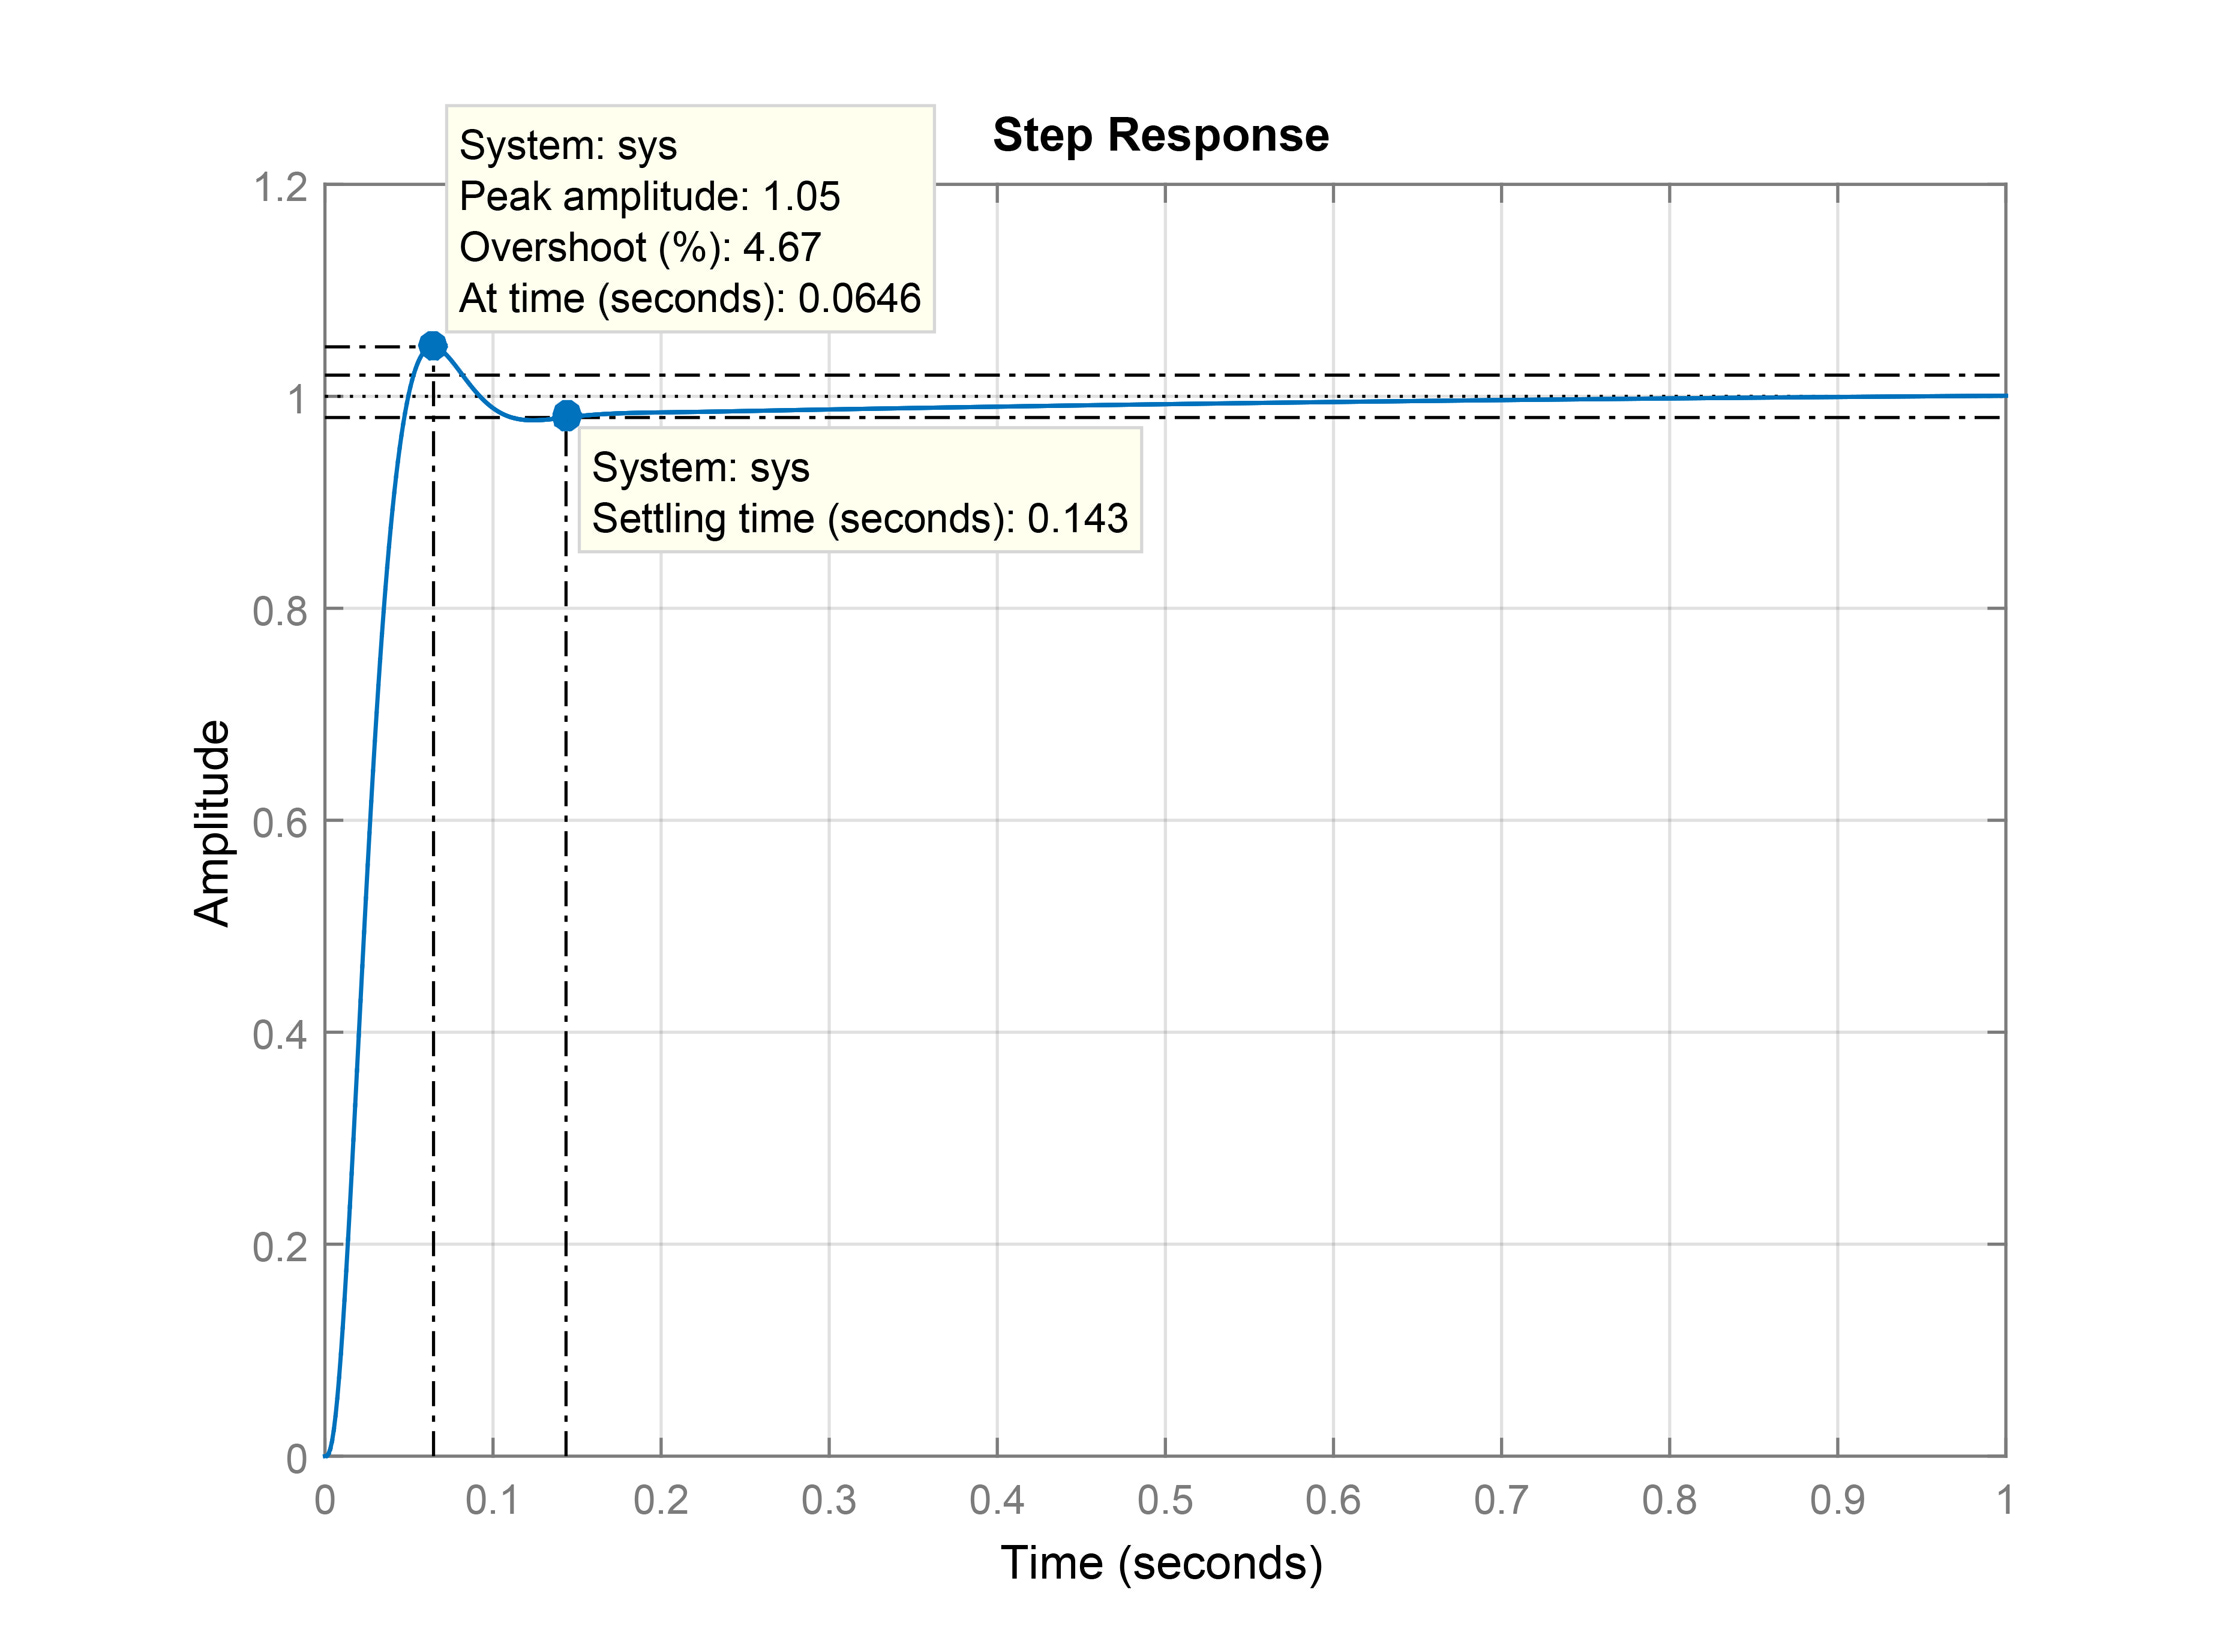
\includegraphics[width=\linewidth]{step_X.pdf}}
\caption{Step response of Y Motor after feedback control}
\label{fig}
\end{figure}  
\subsection{Y motor controller design}
The open loop poles of the X motor plant are:
\begin{itemize}
\item   0
\item  -2.3791
\item  -0.1210
\end{itemize}
The first pole at 0 making the system marginally stable and is the most dominant pole. The root locus of the system is shown in Fig. 7.
\begin{figure}[htbp]
\centerline{\includegraphics[width=\linewidth]{rootlocus_Y.pdf}}
\caption{Zoomed root locus of X Motor without controller}
\label{fig}
\end{figure}
This case is also similar to Y motor. Thus, applying 2nd order Lead compensator is used i.e cascading two lead compensator. The tuned parameters through root locus design of the controller is shown in Fig. 8.
\begin{figure}[htbp]
\centerline{\includegraphics[width=\linewidth]{comp_Y.png}}
\caption{Lead compensator tuned parameters for X motor}
\label{fig}
\end{figure} 
The resulting root locus after tuning the compensator is shown in Fig. 9. In which pole zero cancellation removed the effect of dominant poles near to the origin resulting in large gain margin that helped in achieving the desired response.
\begin{figure}[htbp]
\centerline{\includegraphics[width=\linewidth]{rootlocus_Y2.pdf}}
\caption{Zoomed root locus of X Motor with controller}
\label{fig}
\end{figure}
The step response of closed loop X motor system is shown as Fig. 10.
\begin{figure}[htbp]
\centerline{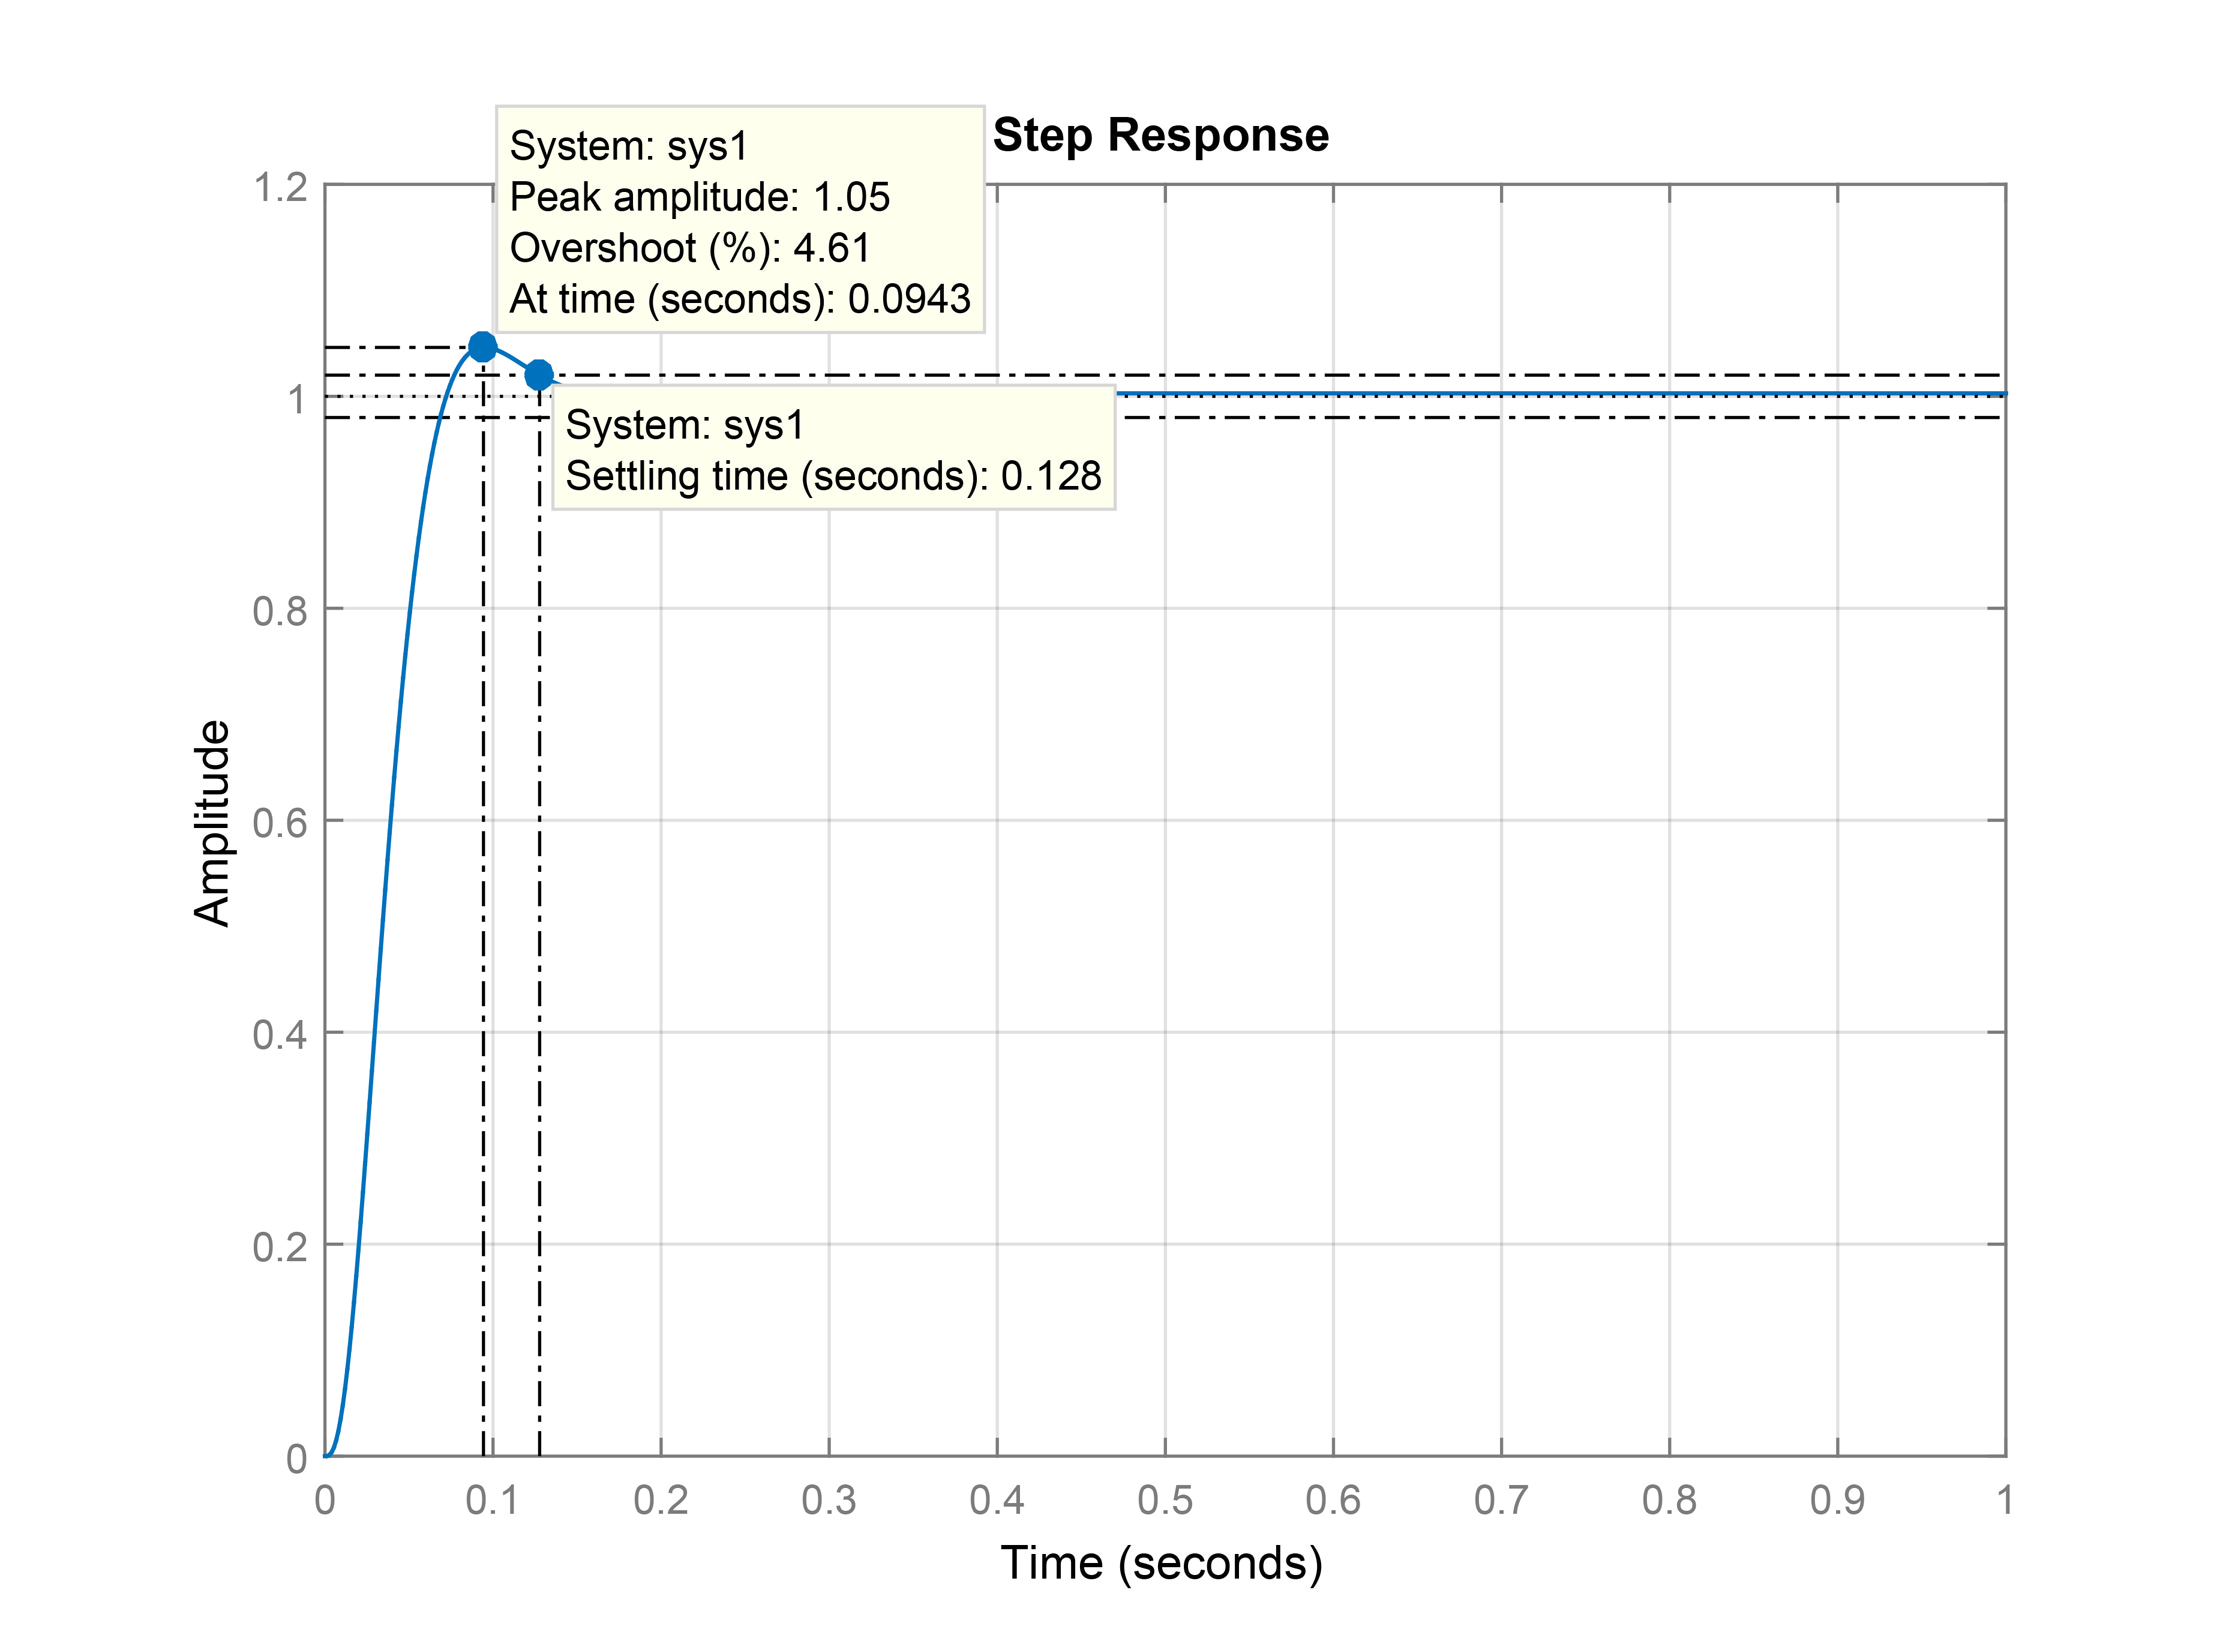
\includegraphics[width=\linewidth]{step_Y.pdf}}
\caption{Step response of X Motor after feedback control}
\label{fig}
\end{figure}

\subsection{Z motor controller design}
The open loop poles of the Z motor plant are:
\begin{itemize}
\item  0
\item  -2.0170
\item  -0.4830
\end{itemize}
The first pole at 0 making the system marginally stable and is the most dominant pole. The root locus of the system is shown in Fig. 11.
\begin{figure}[htbp]
\centerline{\includegraphics[width=\linewidth]{rootlocus_Z.pdf}}
\caption{Zoomed root locus of Z Motor without controller}
\label{fig}
\end{figure}
This case is also similar to X and Y motor. Thus, applying 2nd order Lead compensator is used i.e cascading two lead compensator. The tuned parameters through root locus design of the controller is shown in Fig. 12.
\begin{figure}[htbp]
\centerline{\includegraphics[width=\linewidth]{comp_Z.png}}
\caption{Lead compensator tuned parameters for Z motor}
\label{fig}
\end{figure} 
The resulting root locus after tuning the compensator is shown in Fig. 13. In which pole zero cancellation removed the effect of dominant poles near to the origin resulting in large gain margin that helped in achieving the desired response.
\begin{figure}[htbp]
\centerline{\includegraphics[width=\linewidth]{rootlocus_Z2.pdf}}
\caption{Zoomed root locus of Z Motor with controller}
\label{fig}
\end{figure}
The step response of closed loop Z motor system is shown as Fig. 14.
\begin{figure}[htbp]
\centerline{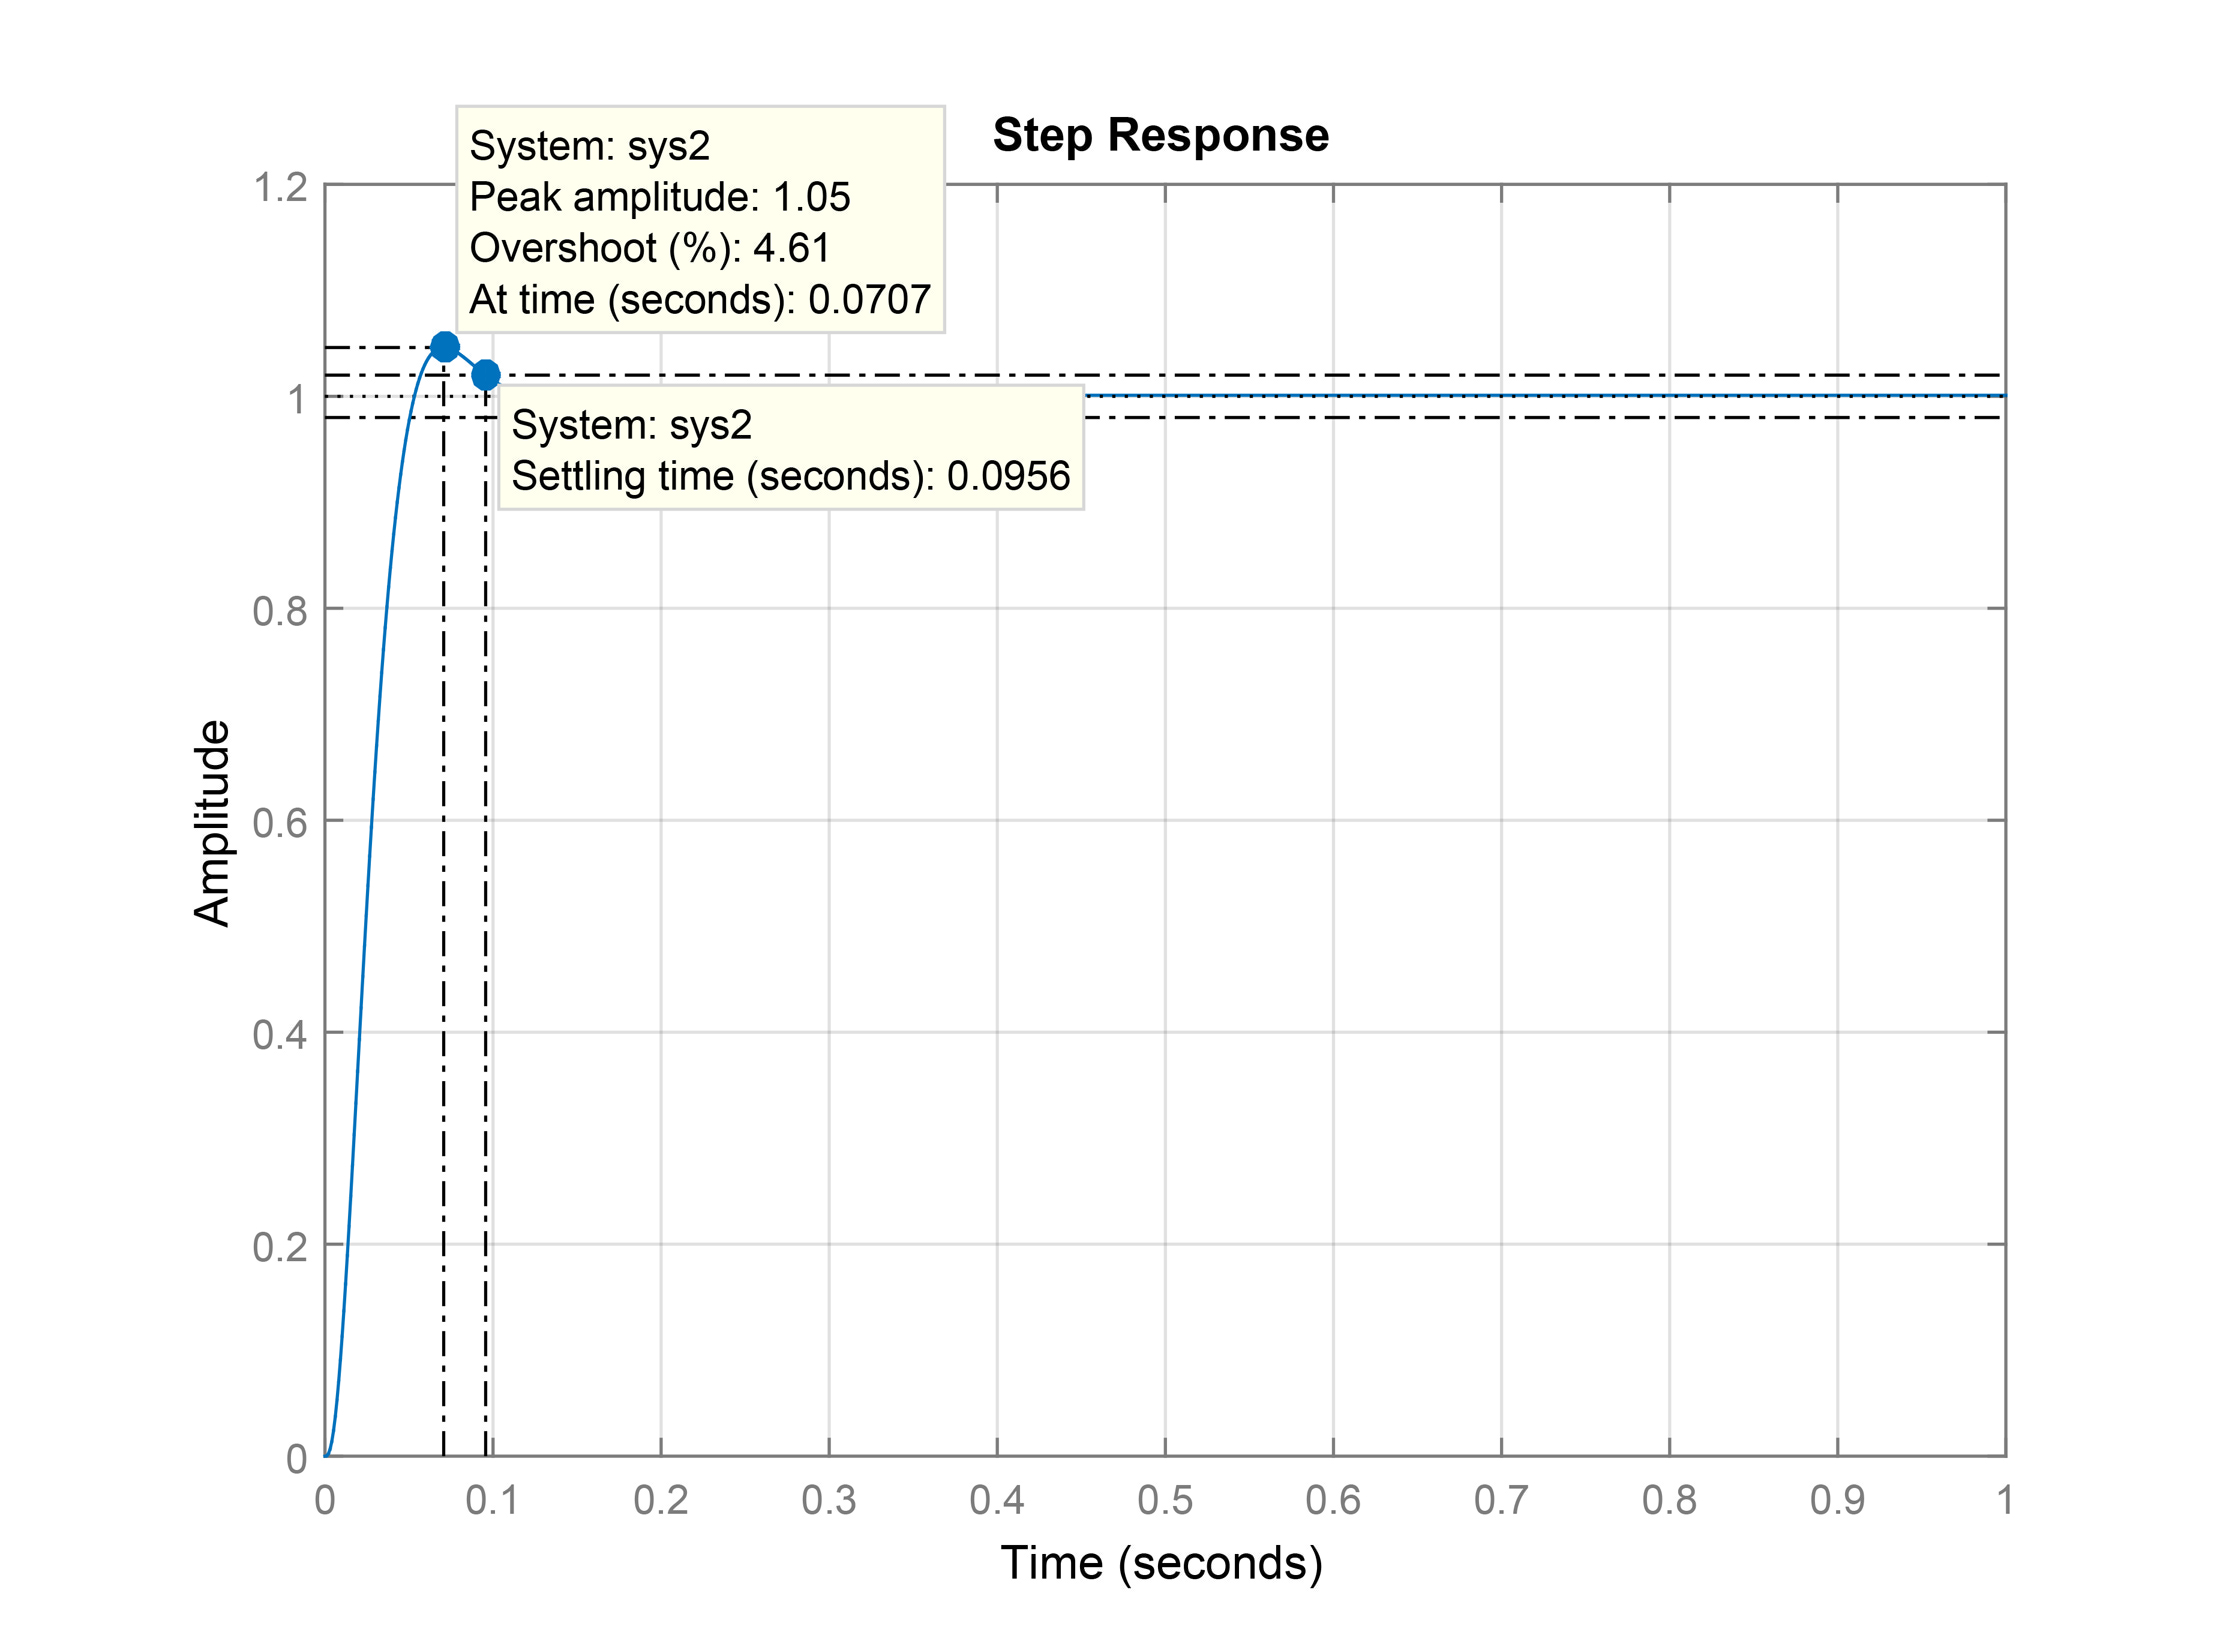
\includegraphics[width=\linewidth]{step_Z.pdf}}
\caption{Step response of Z Motor after feedback control}
\label{fig}
\end{figure}

\subsection{Square wave response on controlled system in Simulink}
Applying continuous step input i.e. square waves using pulse generator having period of 3 seconds and pulse width of 50\%. The output response to the square wave is shown in Fig. 15.
\begin{figure}[htbp]
\centerline{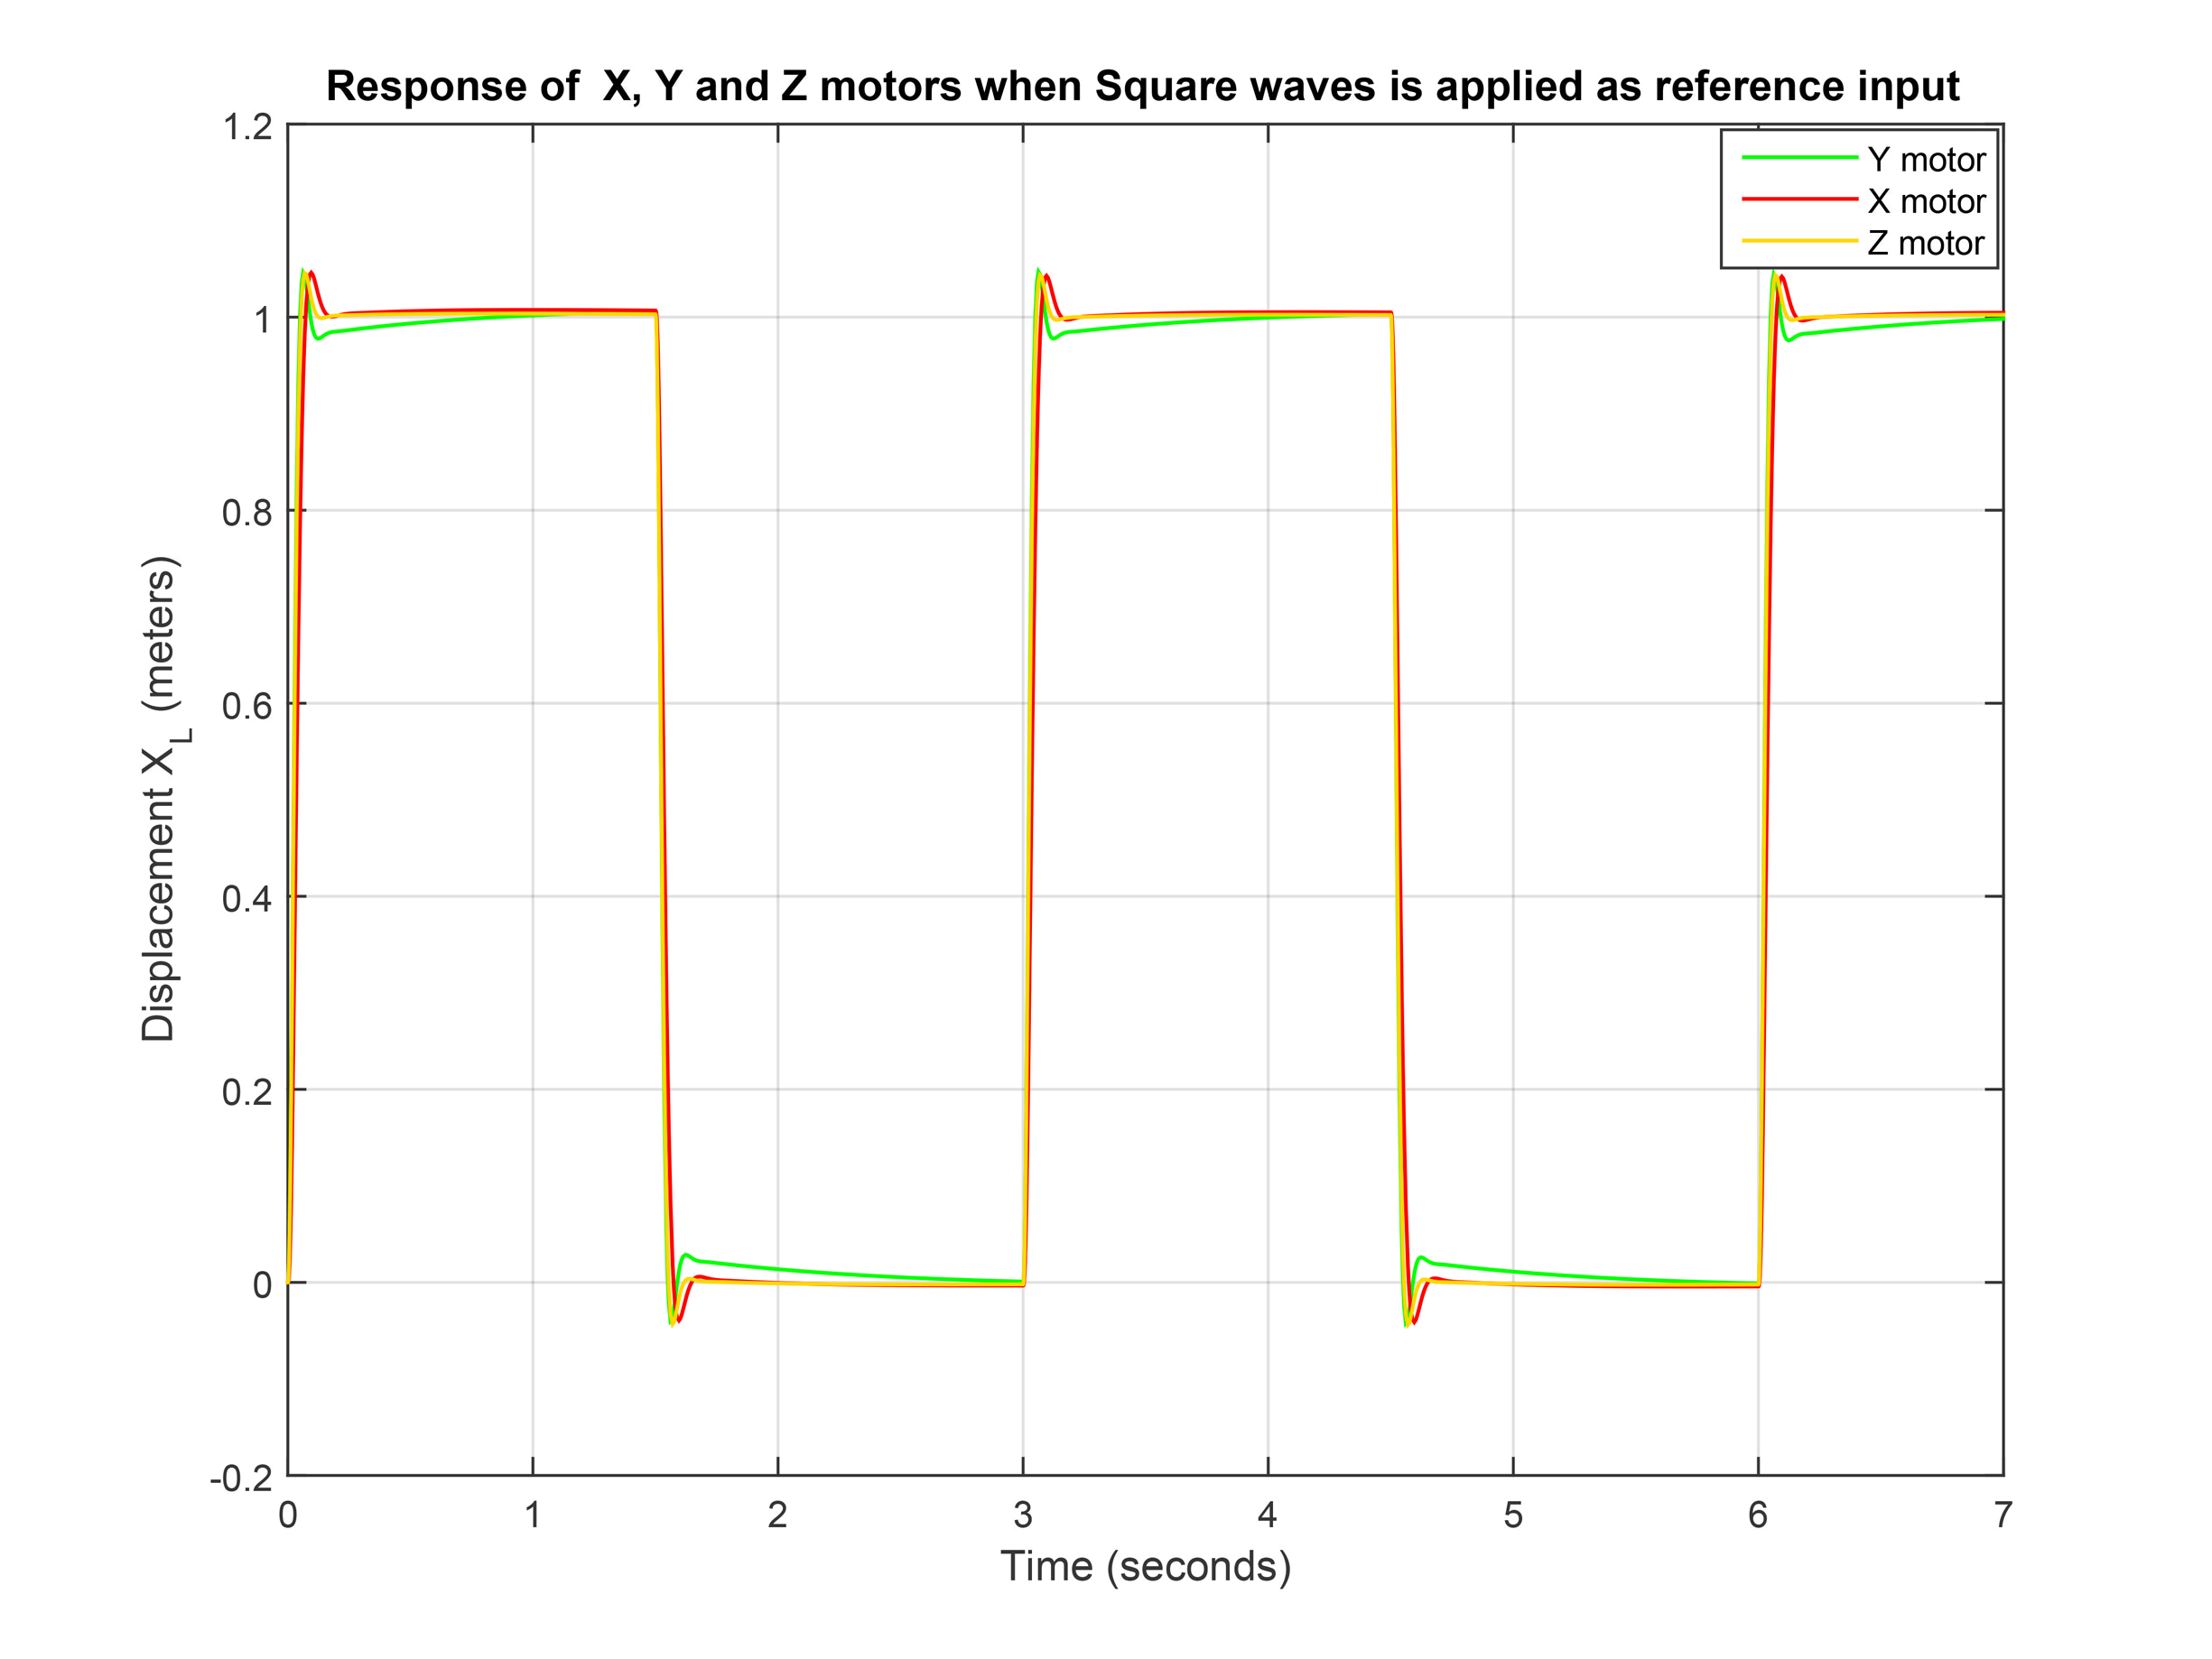
\includegraphics[width=\linewidth]{square.pdf}}
\caption{Response of  X, Y and Z motors when Square waves is applied as reference input}
\label{fig}
\end{figure}
\subsection{Effect of constant disturbance on output}
Applying constant disturbance of 5N does not effect the output response of the system as shown in Fig. 16, which means the feedback controller of every motor can compensate the effect of the applied disturbance. 
\begin{figure}[htbp]
\centerline{\includegraphics[width=\linewidth]{dis_out.pdf}}
\caption{Response of  X, Y and Z motors when disturbance of 5N is applied}
\label{fig}
\end{figure}
\\ Moreover, a comparative plot of step response with and without disturbance is shown in Fig. 17. But a constant force of more than 100N results in slight deviation from the reference input as shown in Fig. 18 which is zoomed to 300\%.
\begin{figure}[htbp]
\centerline{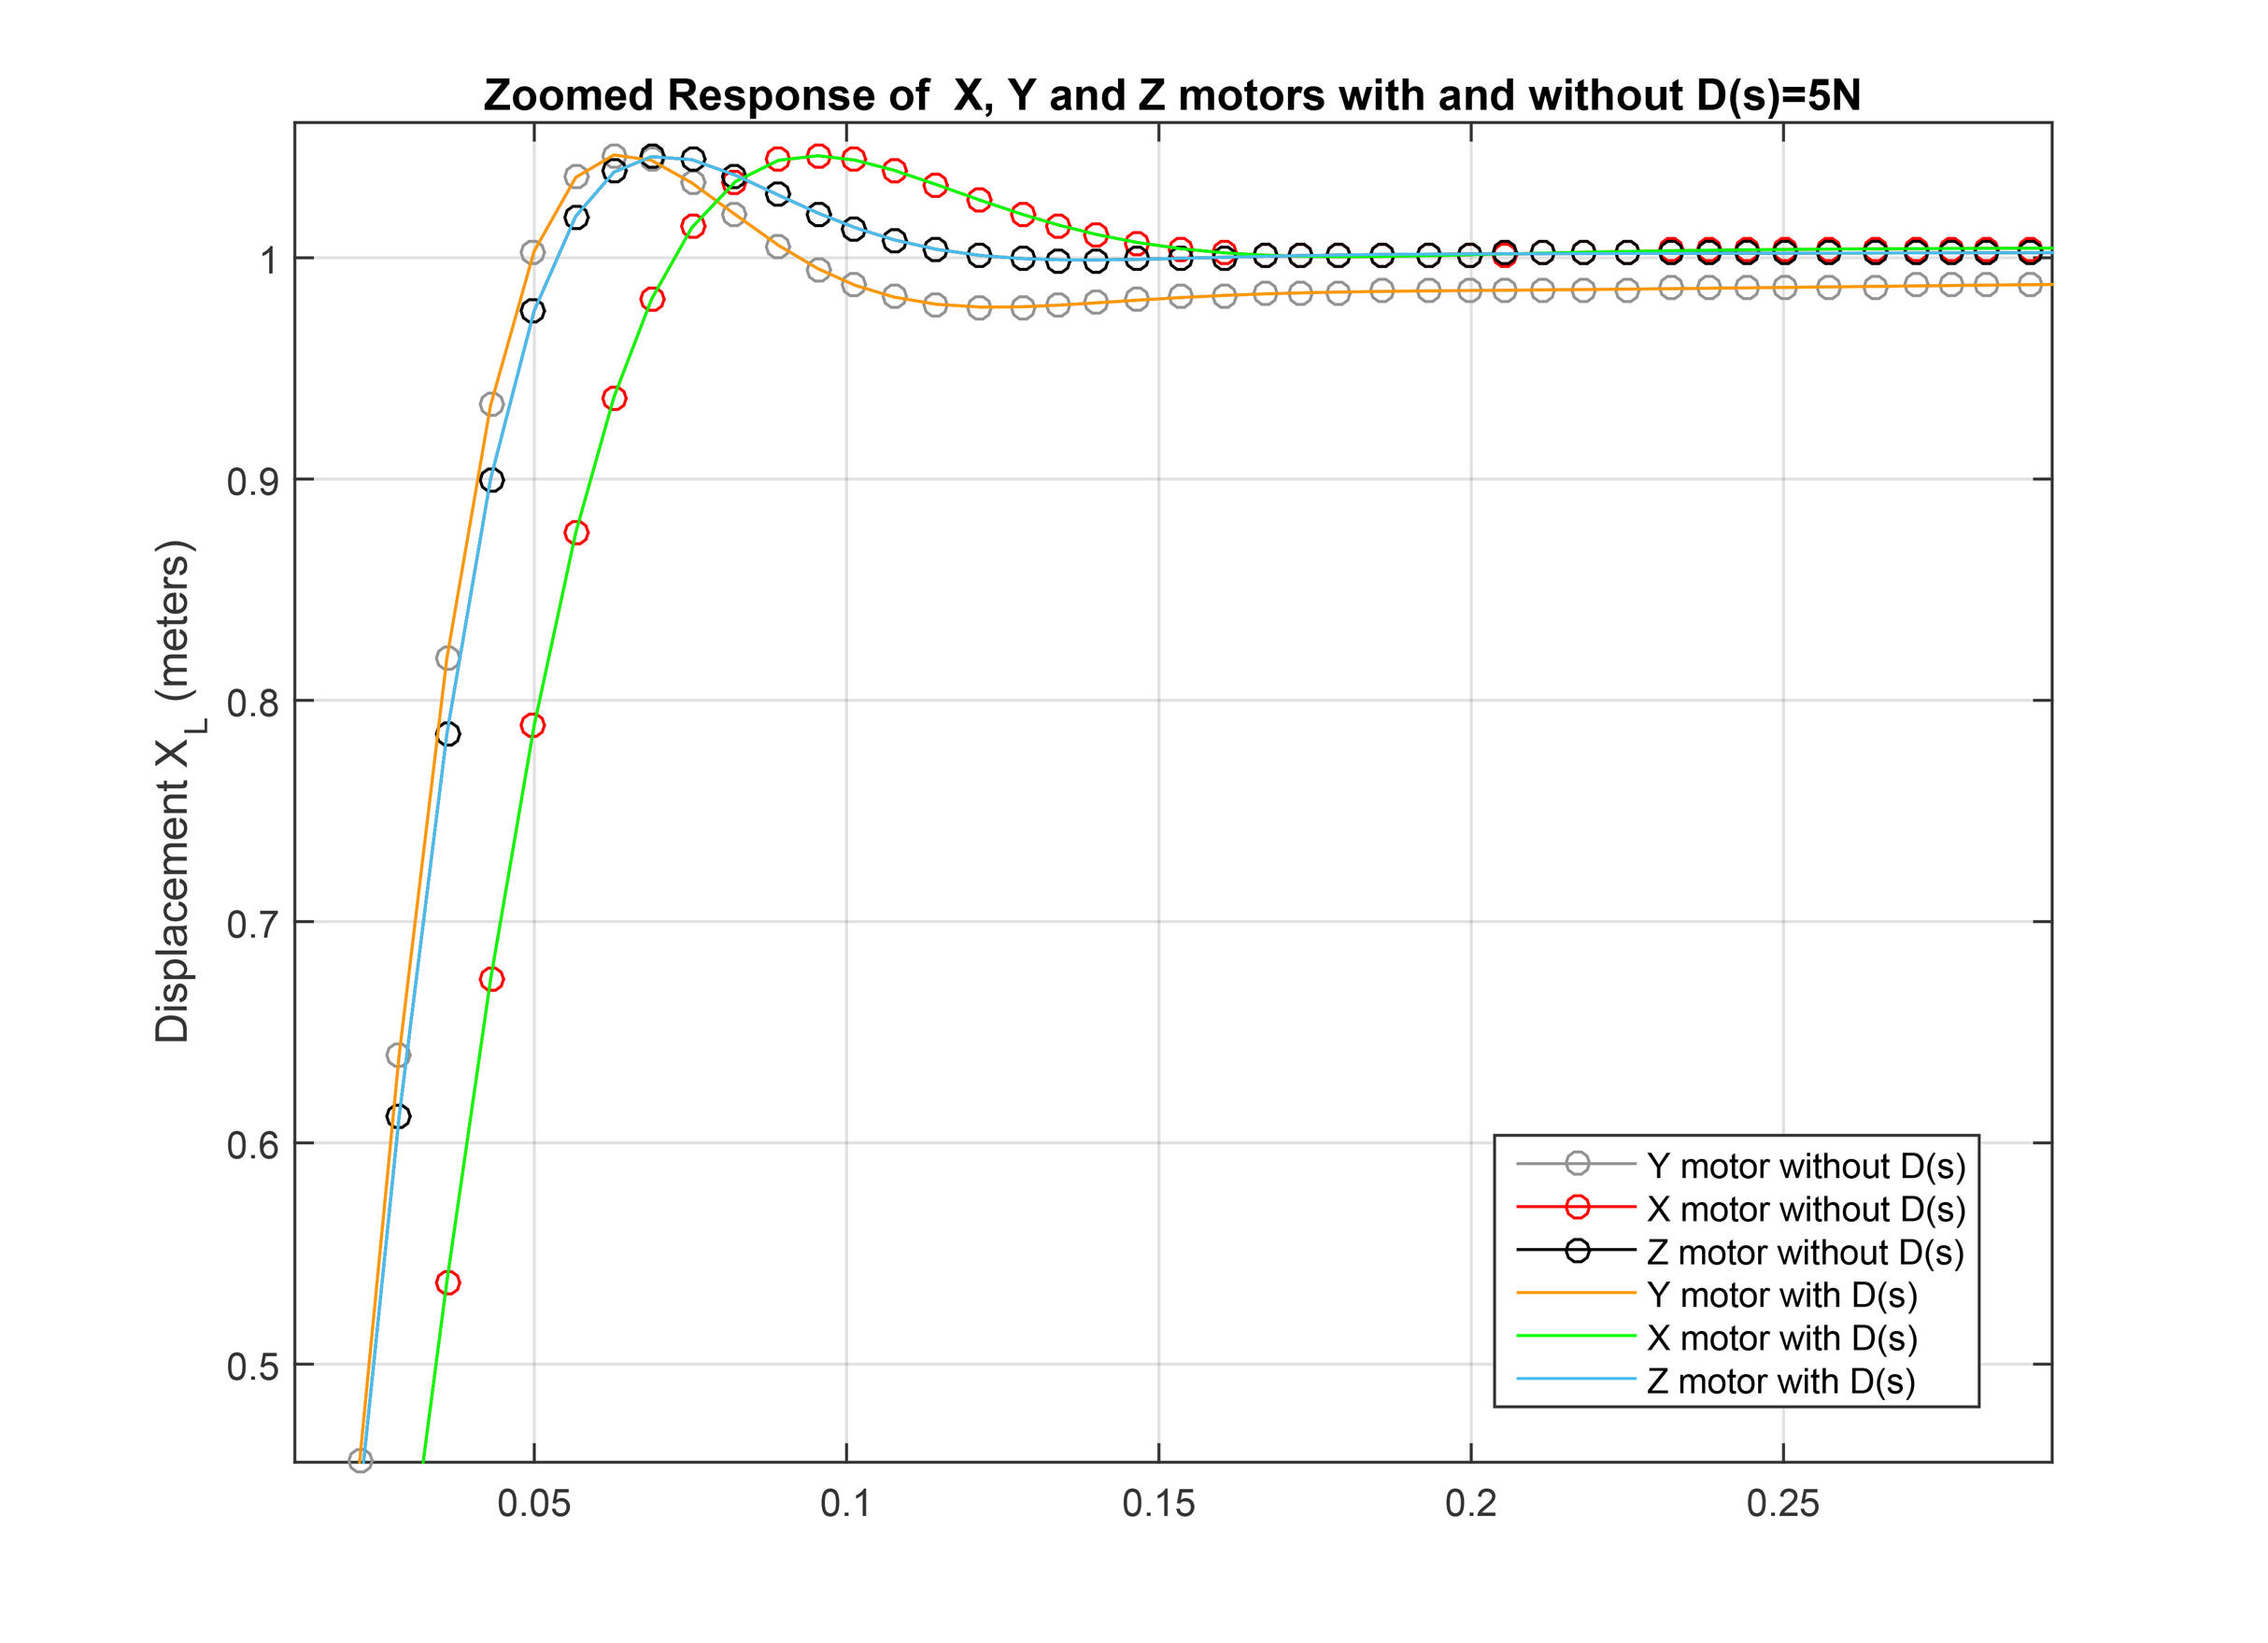
\includegraphics[width=\linewidth]{d_with_No.pdf}}
\caption{Zoomed Response of  X, Y and Z motors with and without disturbance}
\label{fig}
\end{figure}
\begin{figure}[htbp]
\centerline{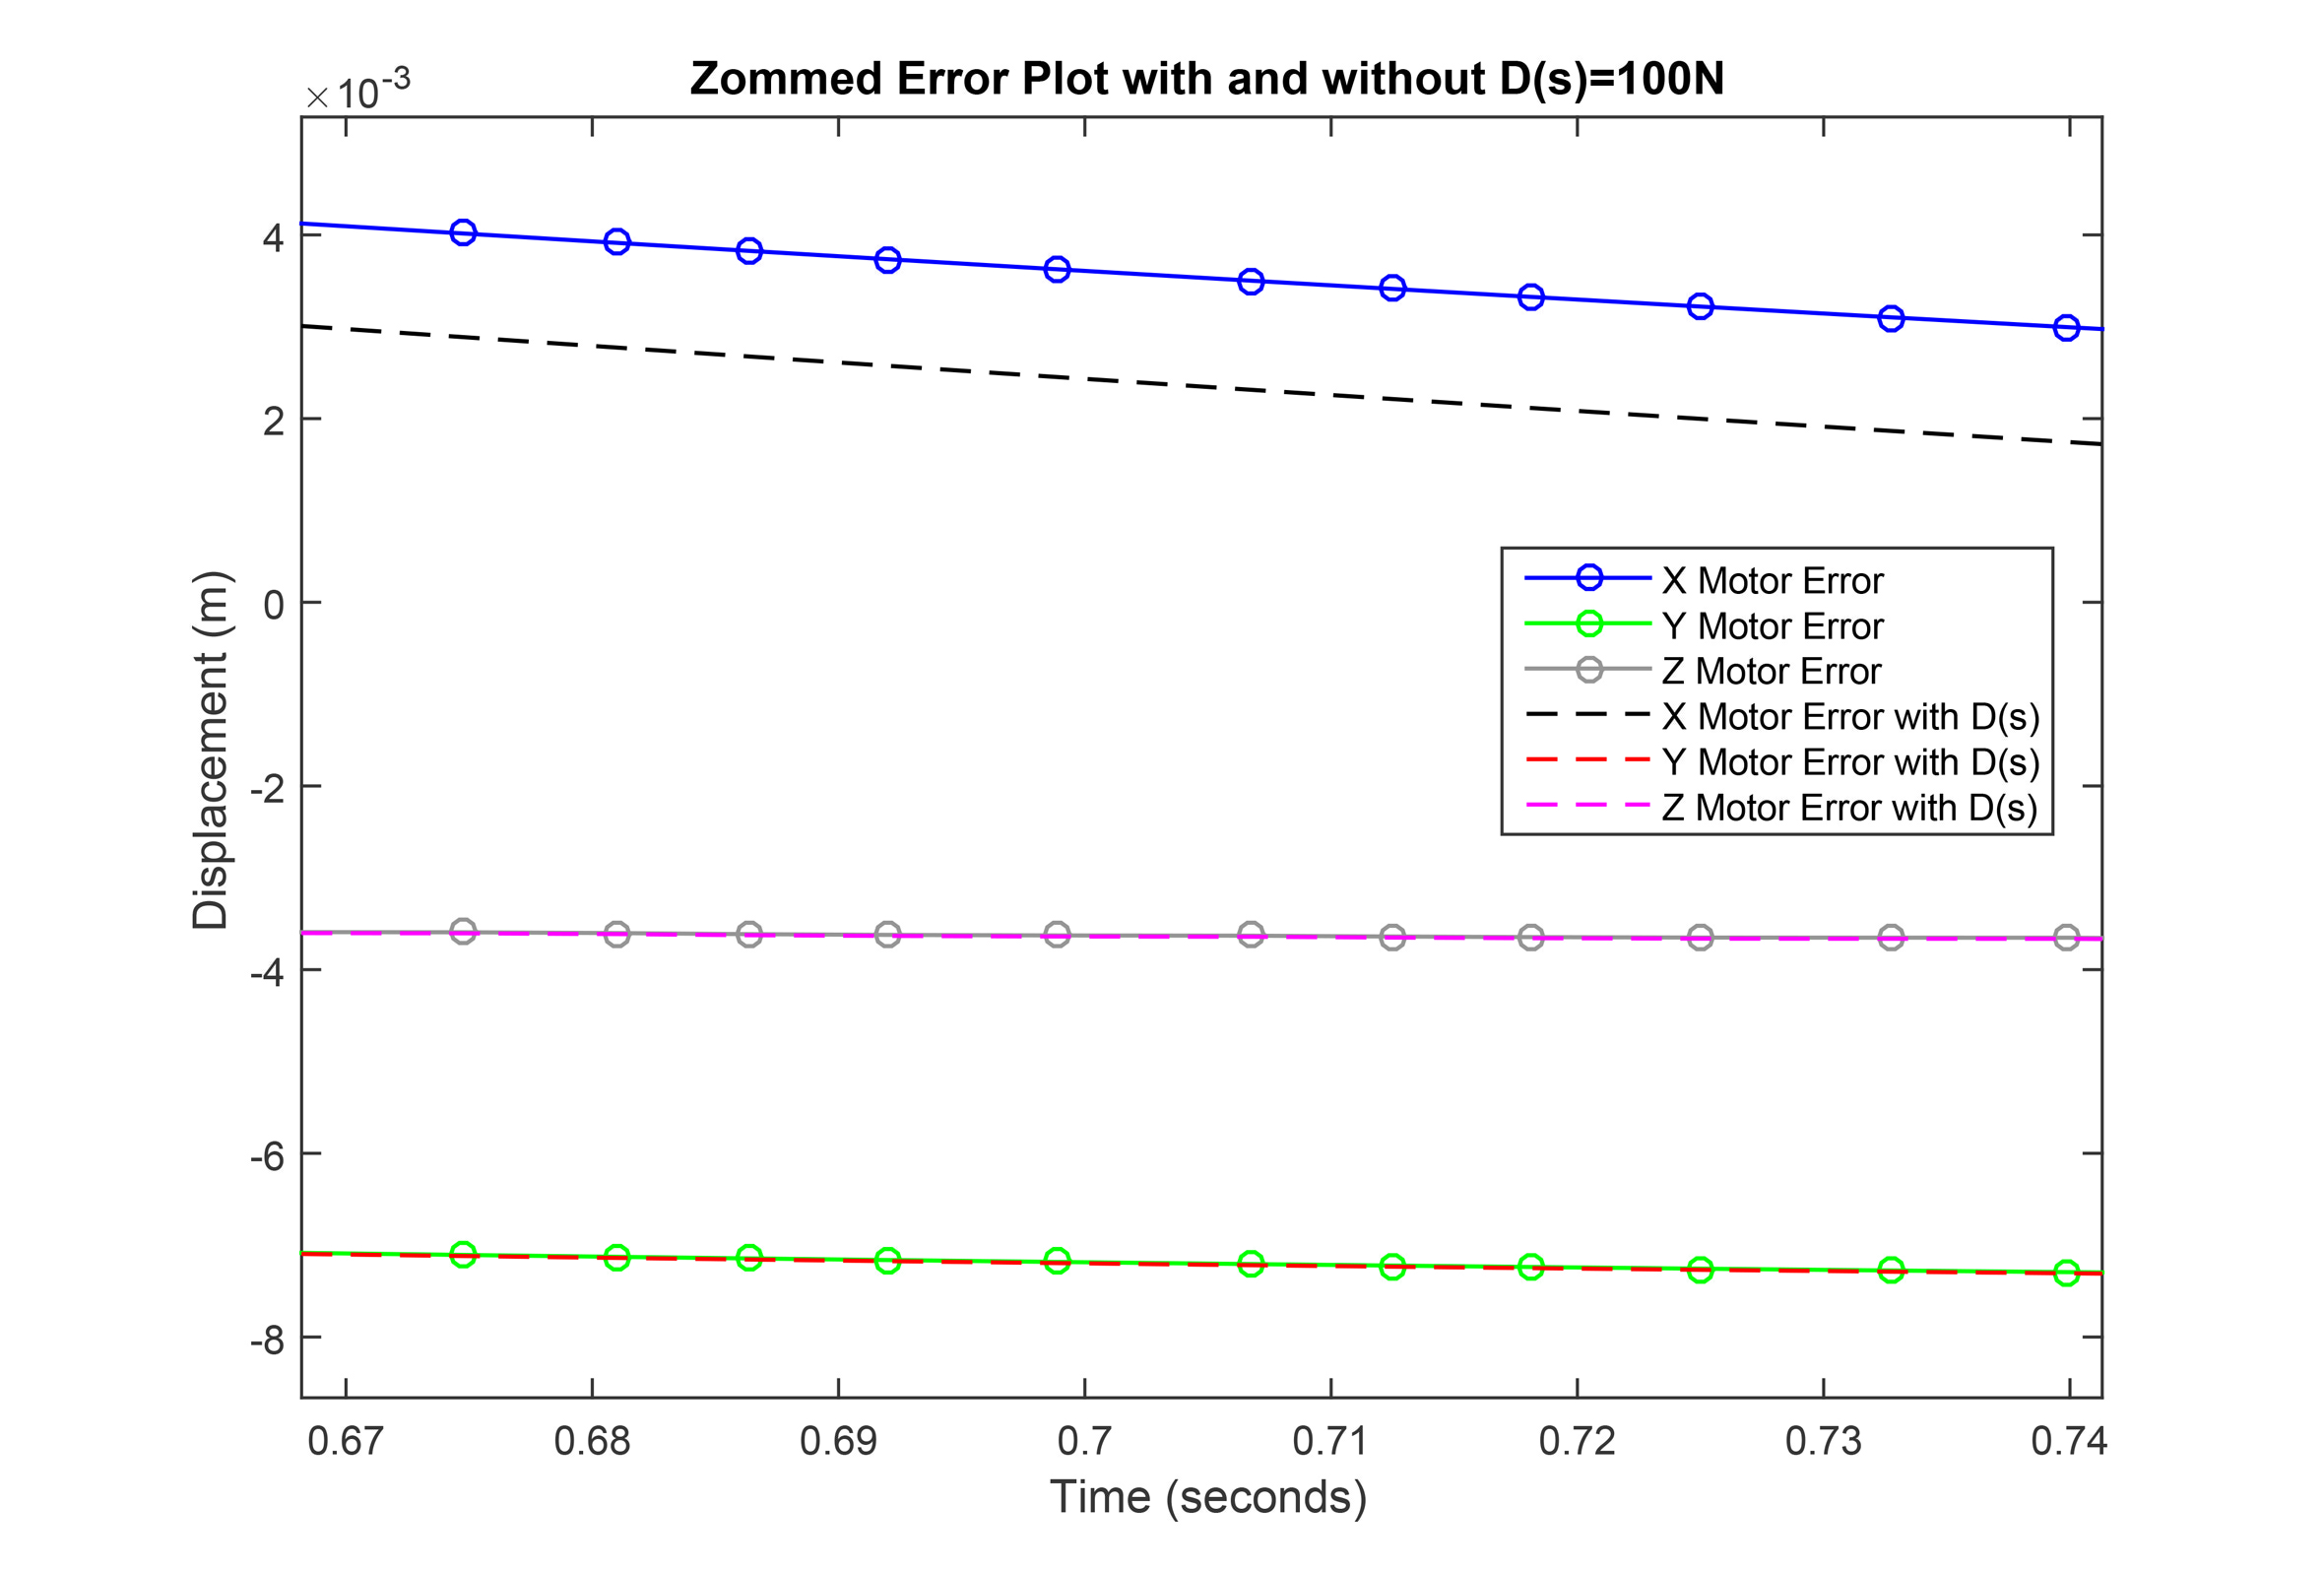
\includegraphics[width=\linewidth]{Err_plot_100N.pdf}}
\caption{300\% zoomed response of  X, Y and Z motors with and without D(s)=100N}
\label{fig}
\end{figure}
\section{3D printing without disturbance}
The following MATLAB code has been used to read data from pseudo .stl file and saving as .mat file for further use.
\begin{lstlisting}[frame=single][language=MATLAB]
dataset=xlsread('pseudo stl file data.xlsx','CakeRaw');% read excel file

x=dataset(1:155,2)%specify rows and columns to read from the file
y=dataset(1:155,3)
z=dataset(1:155,4)
dispense=dataset(:,5)
stop=dataset(:,6)
incr=dataset(1:155,7)

save ('read_cakeRaw.mat', 'x','y','z', 'incr') %saving variables in .mat file for further use 
\end{lstlisting}
Similar code as above has been used to read all the spread sheets from excel file and save it as .mat file.\\ Following code hase been used to simulate the model in Simulink by giving input from MATLAB script and taking output back into MATLAB script and plot it.  Error tolerance hasn't been catered because the error was already below 0.05 and unsynchronization of Simulink time with MATLAB function code loops. Moreover, the input to the simulink model is exactly after 1 second as incr in .stl is treated as time axis, which is greater than the settling time, therefore, the output printed object is doesn't show any large variation.
\begin{lstlisting}[frame=single][language=MATLAB]
load read_cylinder.mat %load .mat file

simin_x=[incr,x]; %passing data to Workspace as Timeseries, where incr is time and x are coordinates  for X Mator
simin_y=[incr,y];
simin_z=[incr,z];

sim('temp2',length(incr)); %running simulation temp2.mdl with simulation time equal to the time scale of .stl file

plot3(simout_x,simout_y,simout_z) %plot 3D on data obtained from ToWorkSpace block of simulink

title('Cylinder with constant D(s)')
xlabel('x-axis (meters)')
ylabel('y-axis (meters)')
zlabel('z-axis (meters)')
grid on

figure
plot(err_x) %plot of error from E(s) in feedback loop of Motor X
title('Motor X Error Plot with D(s)')
ylabel('Displacement (m)')
grid on

figure
plot (err_y) %plot of error from E(s) in feedback loop of Motor Y
title('Motor Y Error Plot with D(s)')
ylabel('Displacement (m)')
grid on

figure
plot (err_z) %plot of error from E(s) in feedback loop of Motor Z
ylabel('Displacement (m)')
title('Motor Z Error Plot with D(s)')
grid on

\end{lstlisting}
\subsection{3d printing of Rectangle}
The 3d plot of Rectangle shown in Fig. 19 without any disturbance.
\begin{figure}[htbp]
\centerline{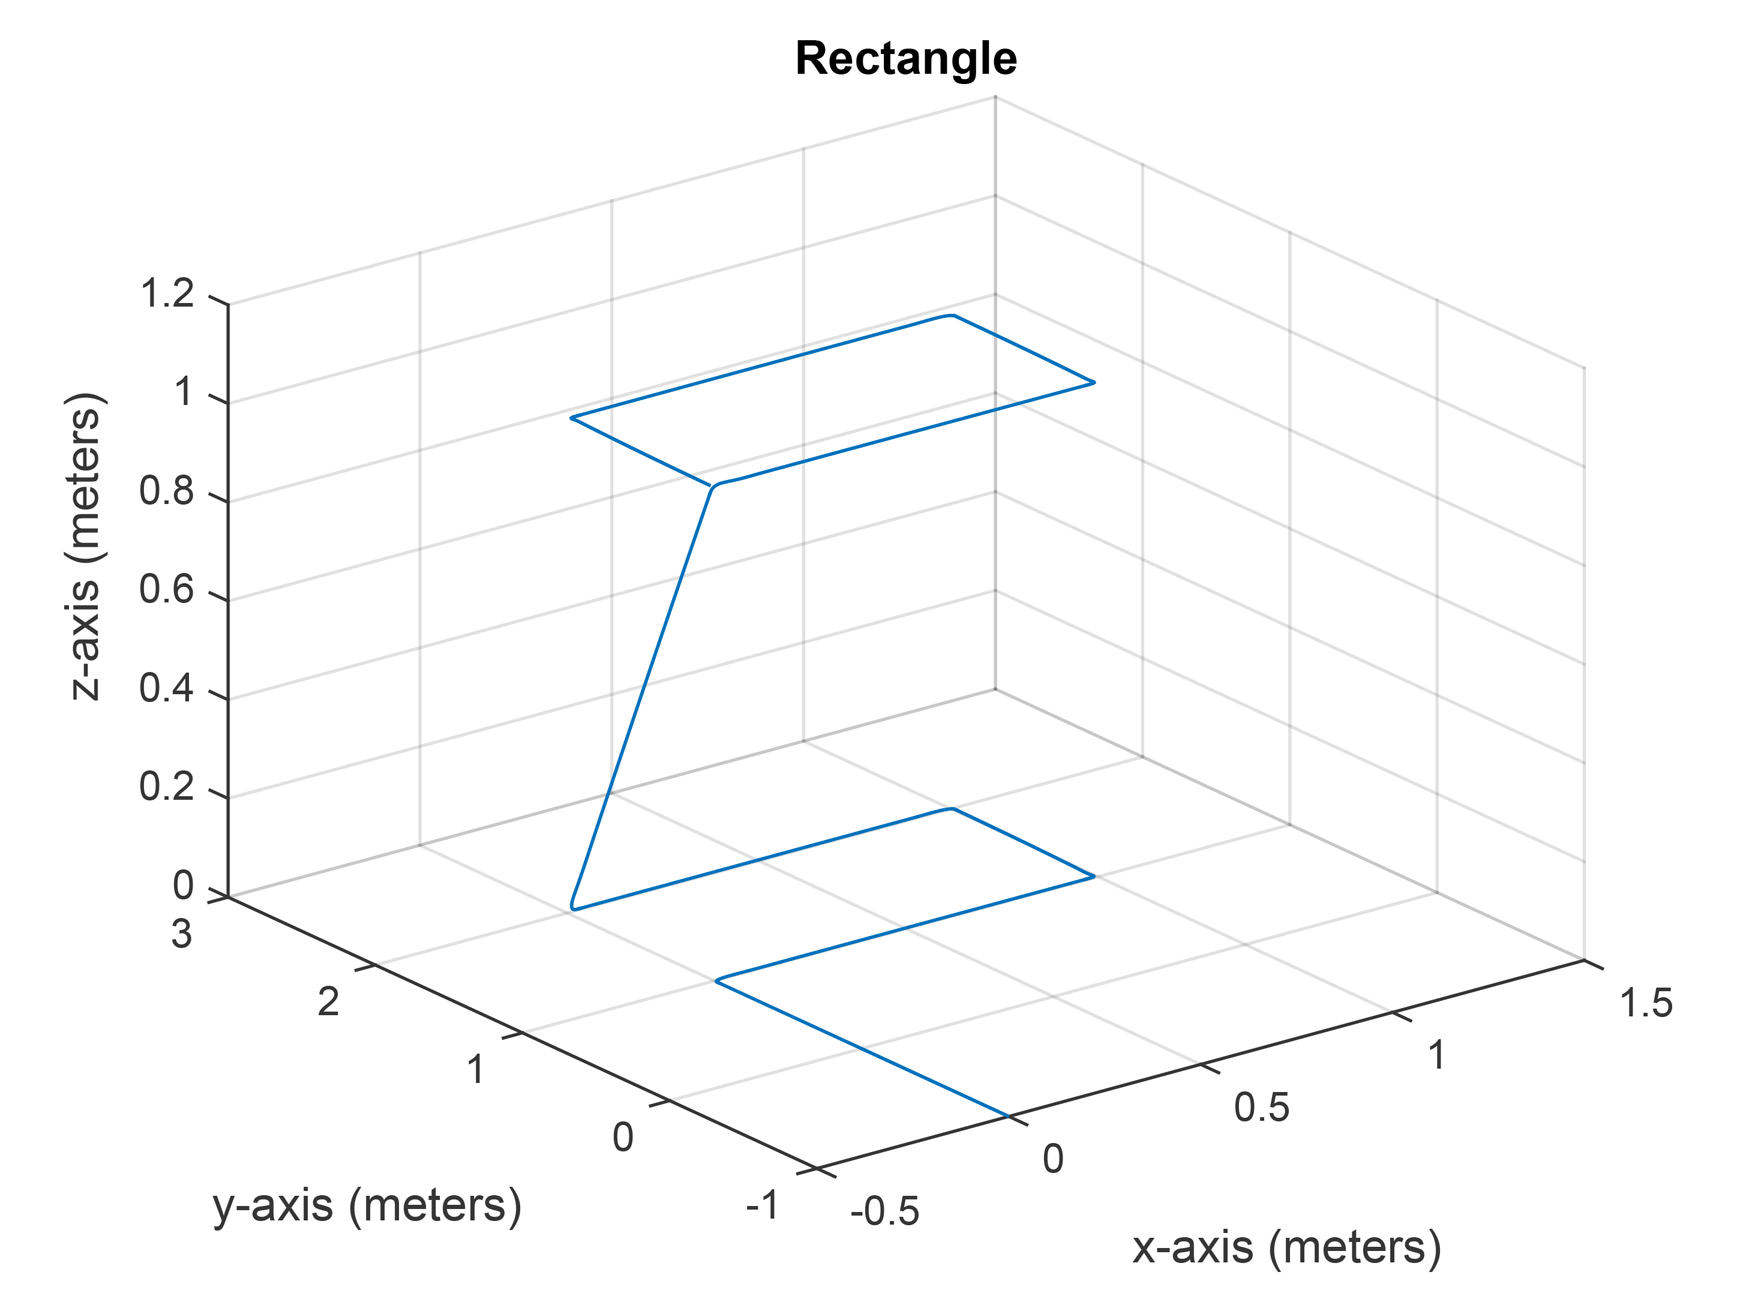
\includegraphics[width=\linewidth]{rectangle_print.pdf}}
\caption{Rectangle 3d plot without disturbance}
\label{fig}
\end{figure}
The edges are slightly circular when the figure is zoomed because of error tolerance. The error plots of X, Y and Z motors in case of rectangle in shown Fig. 20, Fig. 21 and Fig. 22 respectively.
 \begin{figure}[htbp]
\centerline{\includegraphics[width=\linewidth]{rectangle_errx.pdf}}
\caption{X motor error plot while printing Rectangle}
\label{fig}
\end{figure}\begin{figure}[htbp]
\centerline{\includegraphics[width=\linewidth]{rectangle_erry.pdf}}
\caption{Y motor error plot while printing Rectangle}
\label{fig}
\end{figure}\begin{figure}[htbp]
\centerline{\includegraphics[width=\linewidth]{rectangle_errz.pdf}}
\caption{Z motor error plot while printing Rectangle}
\label{fig}
\end{figure}
\subsection{3d printing of Cylinder}
The 3d plot of Cylinder shown in Fig. 23 without any disturbance.
\begin{figure}[htbp]
\centerline{\includegraphics[width=\linewidth]{cylinder_print.pdf}}
\caption{Cylinder 3d plot without disturbance}
\label{fig}
\end{figure}
No error can be visualized in cylinder as it has no sharp edges for further eleboration the error plots of X, Y and Z motors are shown Fig. 24, Fig. 25 and Fig. 26 respectively.
 \begin{figure}[htbp]
\centerline{\includegraphics[width=\linewidth]{cylinder_errx.pdf}}
\caption{X motor error plot while printing Cylinder}
\label{fig}
\end{figure}\begin{figure}[htbp]
\centerline{\includegraphics[width=\linewidth]{cylinder_erry.pdf}}
\caption{Y motor error plot while printing Cylinder}
\label{fig}
\end{figure}\begin{figure}[htbp]
\centerline{\includegraphics[width=\linewidth]{cylinder_errz.pdf}}
\caption{Z motor error plot while printing Cylinder}
\label{fig}
\end{figure}
\subsection{3d printing of Cube}
The 3d plot of Cube shown in Fig. 27 without any disturbance.
\begin{figure}[htbp]
\centerline{\includegraphics[width=\linewidth]{cube_print.pdf}}
\caption{Cube 3d plot without disturbance}
\label{fig}
\end{figure}
The edges of Cube is not sharp enough when the figure is zoomed because of error tolerance. The error plots of X, Y and Z motors in case of Cube in shown Fig. 28, Fig. 29 and Fig. 30 respectively.
 \begin{figure}[htbp]
\centerline{\includegraphics[width=\linewidth]{cube_errx.pdf}}
\caption{X motor error plot while printing Cube}
\label{fig}
\end{figure}\begin{figure}[htbp]
\centerline{\includegraphics[width=\linewidth]{cube_erry.pdf}}
\caption{Y motor error plot while printing Cube}
\label{fig}
\end{figure}\begin{figure}[htbp]
\centerline{\includegraphics[width=\linewidth]{cube_errz.pdf}}
\caption{Z motor error plot while printing Cube}
\label{fig}
\end{figure}
\subsection{3d printing of Pyramid}
The 3d plot of Pyramid shown in Fig. 31 without any disturbance.
\begin{figure}[htbp]
\centerline{\includegraphics[width=\linewidth]{pyramid_print.pdf}}
\caption{Pyramid 3d plot without disturbance}
\label{fig}
\end{figure}
The edges of Pyramid is not sharp enough when the figure is zoomed because of error tolerance. The error plots of X, Y and Z motors in case of Pyramid in shown Fig. 32, Fig. 33 and Fig. 34 respectively.
 \begin{figure}[htbp]
\centerline{\includegraphics[width=\linewidth]{pyramid_errx.pdf}}
\caption{X motor error plot while printing Pyramid}
\label{fig}
\end{figure}\begin{figure}[htbp]
\centerline{\includegraphics[width=\linewidth]{pyramid_erry.pdf}}
\caption{Y motor error plot while printing Pyramid}
\label{fig}
\end{figure}\begin{figure}[htbp]
\centerline{\includegraphics[width=\linewidth]{pyramid_errz.pdf}}
\caption{Z motor error plot while printing Pyramid}
\label{fig}
\end{figure}

\section{3D printing with disturbance of 500N}
\subsection{3d printing of Rectangle with D(s)}
The 3d plot of Rectangle shown in Fig. 35 with a constant disturbance of 500N applied on each X, Y and Z motor.
\begin{figure}[htbp]
\centerline{\includegraphics[width=\linewidth]{rectangle_print_D.pdf}}
\caption{Rectangle 3d plot with D(s)=500N}
\label{fig}
\end{figure}
The edges are slightly circular when the figure is zoomed because of error tolerance. The error plots of X, Y and Z motors in case of rectangle in shown Fig. 36, Fig. 37 and Fig. 38 respectively. Although error increases with disturbance but was quiet small to produce any visual change in the printed object.
 \begin{figure}[htbp]
\centerline{\includegraphics[width=\linewidth]{rectangle_errx_D.pdf}}
\caption{X motor error plot in Rectangle printing with D(s)}
\label{fig}
\end{figure}\begin{figure}[htbp]
\centerline{\includegraphics[width=\linewidth]{rectangle_erry_D.pdf}}
\caption{Y motor error plot while printing Rectangle with D(s)}
\label{fig}
\end{figure}\begin{figure}[htbp]
\centerline{\includegraphics[width=\linewidth]{rectangle_errz_D.pdf}}
\caption{Z motor error plot while printing Rectangle with D(s)}
\label{fig}
\end{figure}
\subsection{3d printing of Cylinder with D(s)}
The 3d plot of Cylinder shown in Fig. 39 without any disturbance.
\begin{figure}[htbp]
\centerline{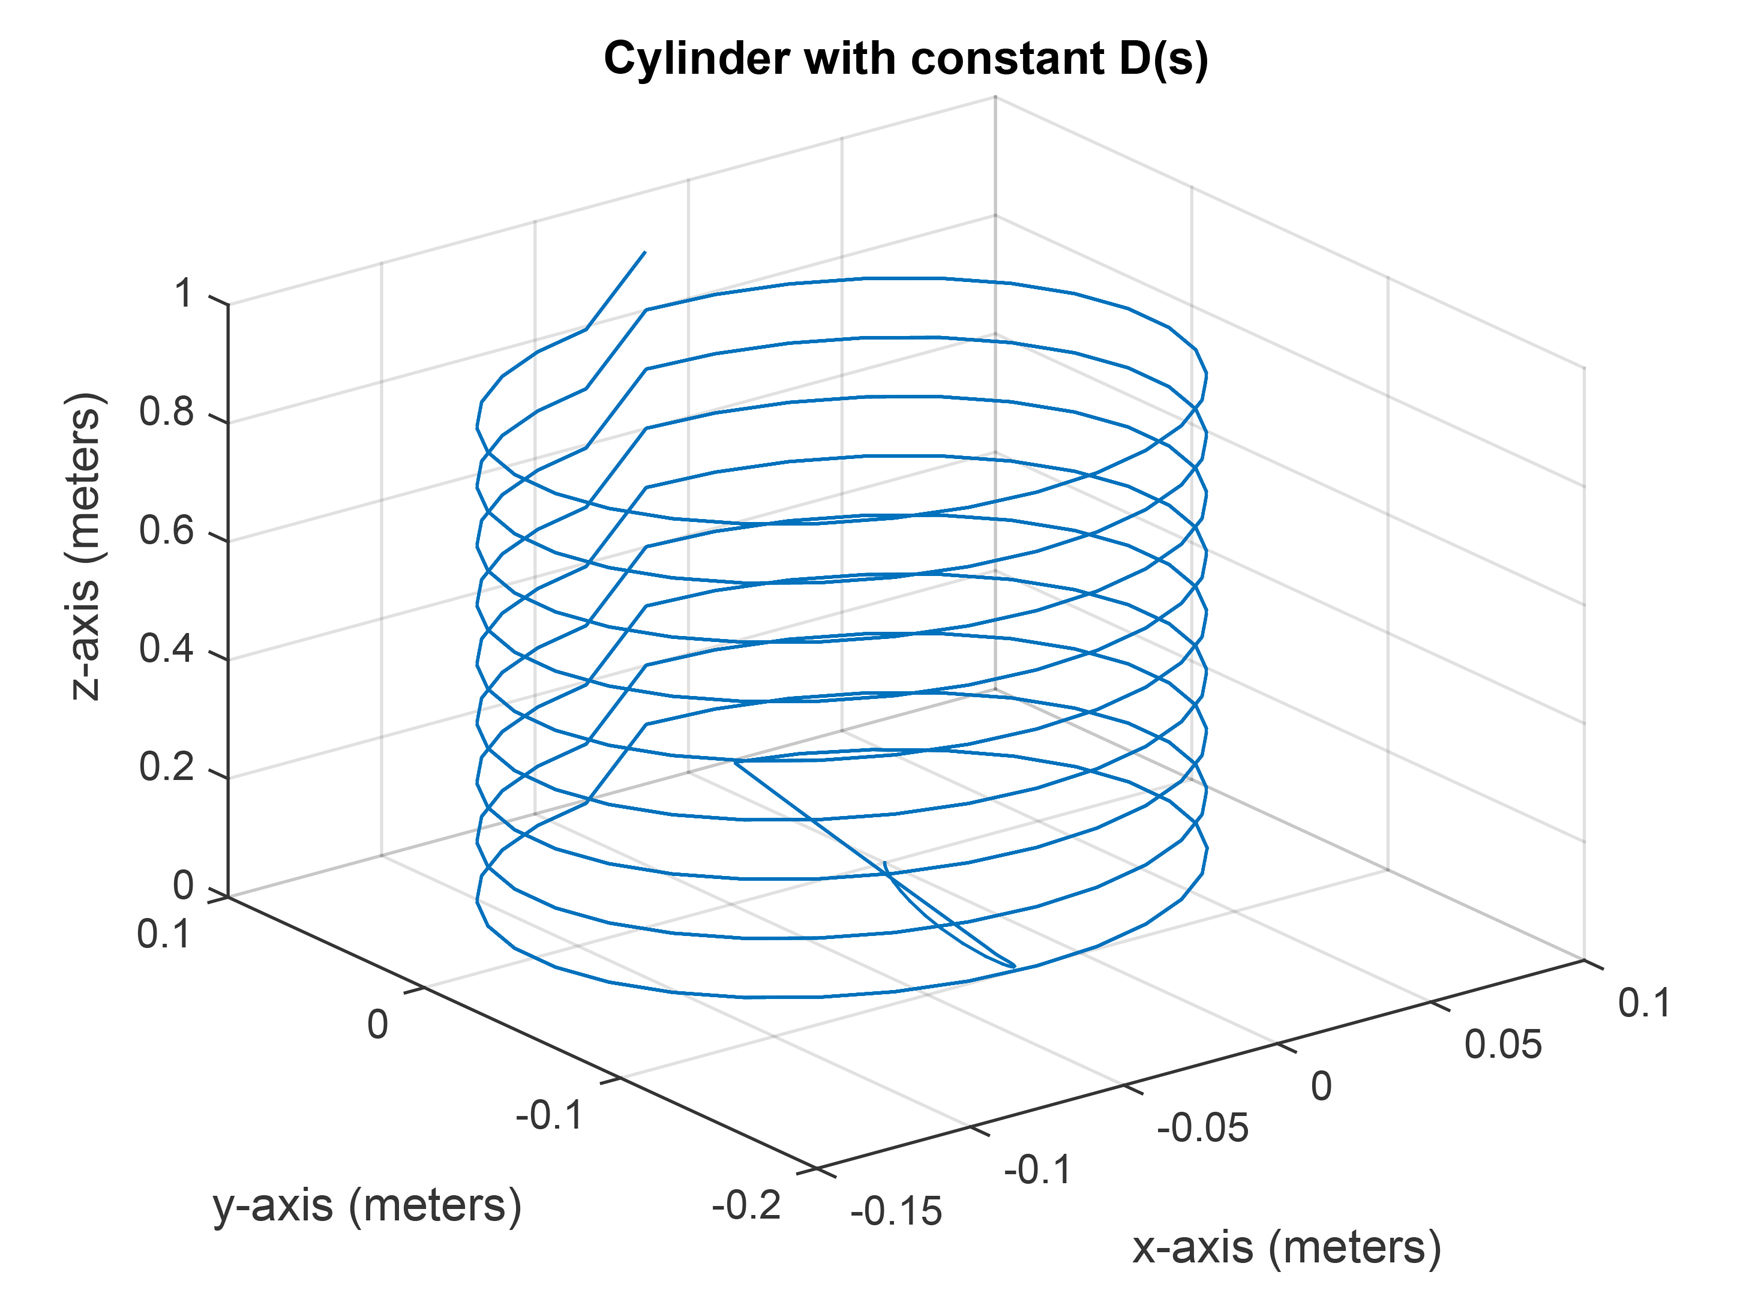
\includegraphics[width=\linewidth]{cylinder_print_D.pdf}}
\caption{Cylinder 3d plot with D(s)=500N}
\label{fig}
\end{figure}
The change in layers of cylinder is not sharp enough  when the figure is zoomed because of error tolerance. The error plots of X, Y and Z motors in case of cylinder in shown Fig. 40, Fig.41 and Fig. 42 respectively. Although error increases with disturbance but was quiet small to produce any visual change in the printed object.
 \begin{figure}[htbp]
\centerline{\includegraphics[width=\linewidth]{cylinder_errx_D.pdf}}
\caption{X motor error plot while printing Cylinder with D(s)}
\label{fig}
\end{figure}\begin{figure}[htbp]
\centerline{\includegraphics[width=\linewidth]{cylinder_erry_D.pdf}}
\caption{Y motor error plot while printing Cylinder with D(s)}
\label{fig}
\end{figure}\begin{figure}[htbp]
\centerline{\includegraphics[width=\linewidth]{cylinder_errz_D.pdf}}
\caption{Z motor error plot while printing Cylinder with D(s)}
\label{fig}
\end{figure}
\subsection{3d printing of Cube with D(s)}
The 3d plot of Cube shown in Fig. 43 without any disturbance.
\begin{figure}[htbp]
\centerline{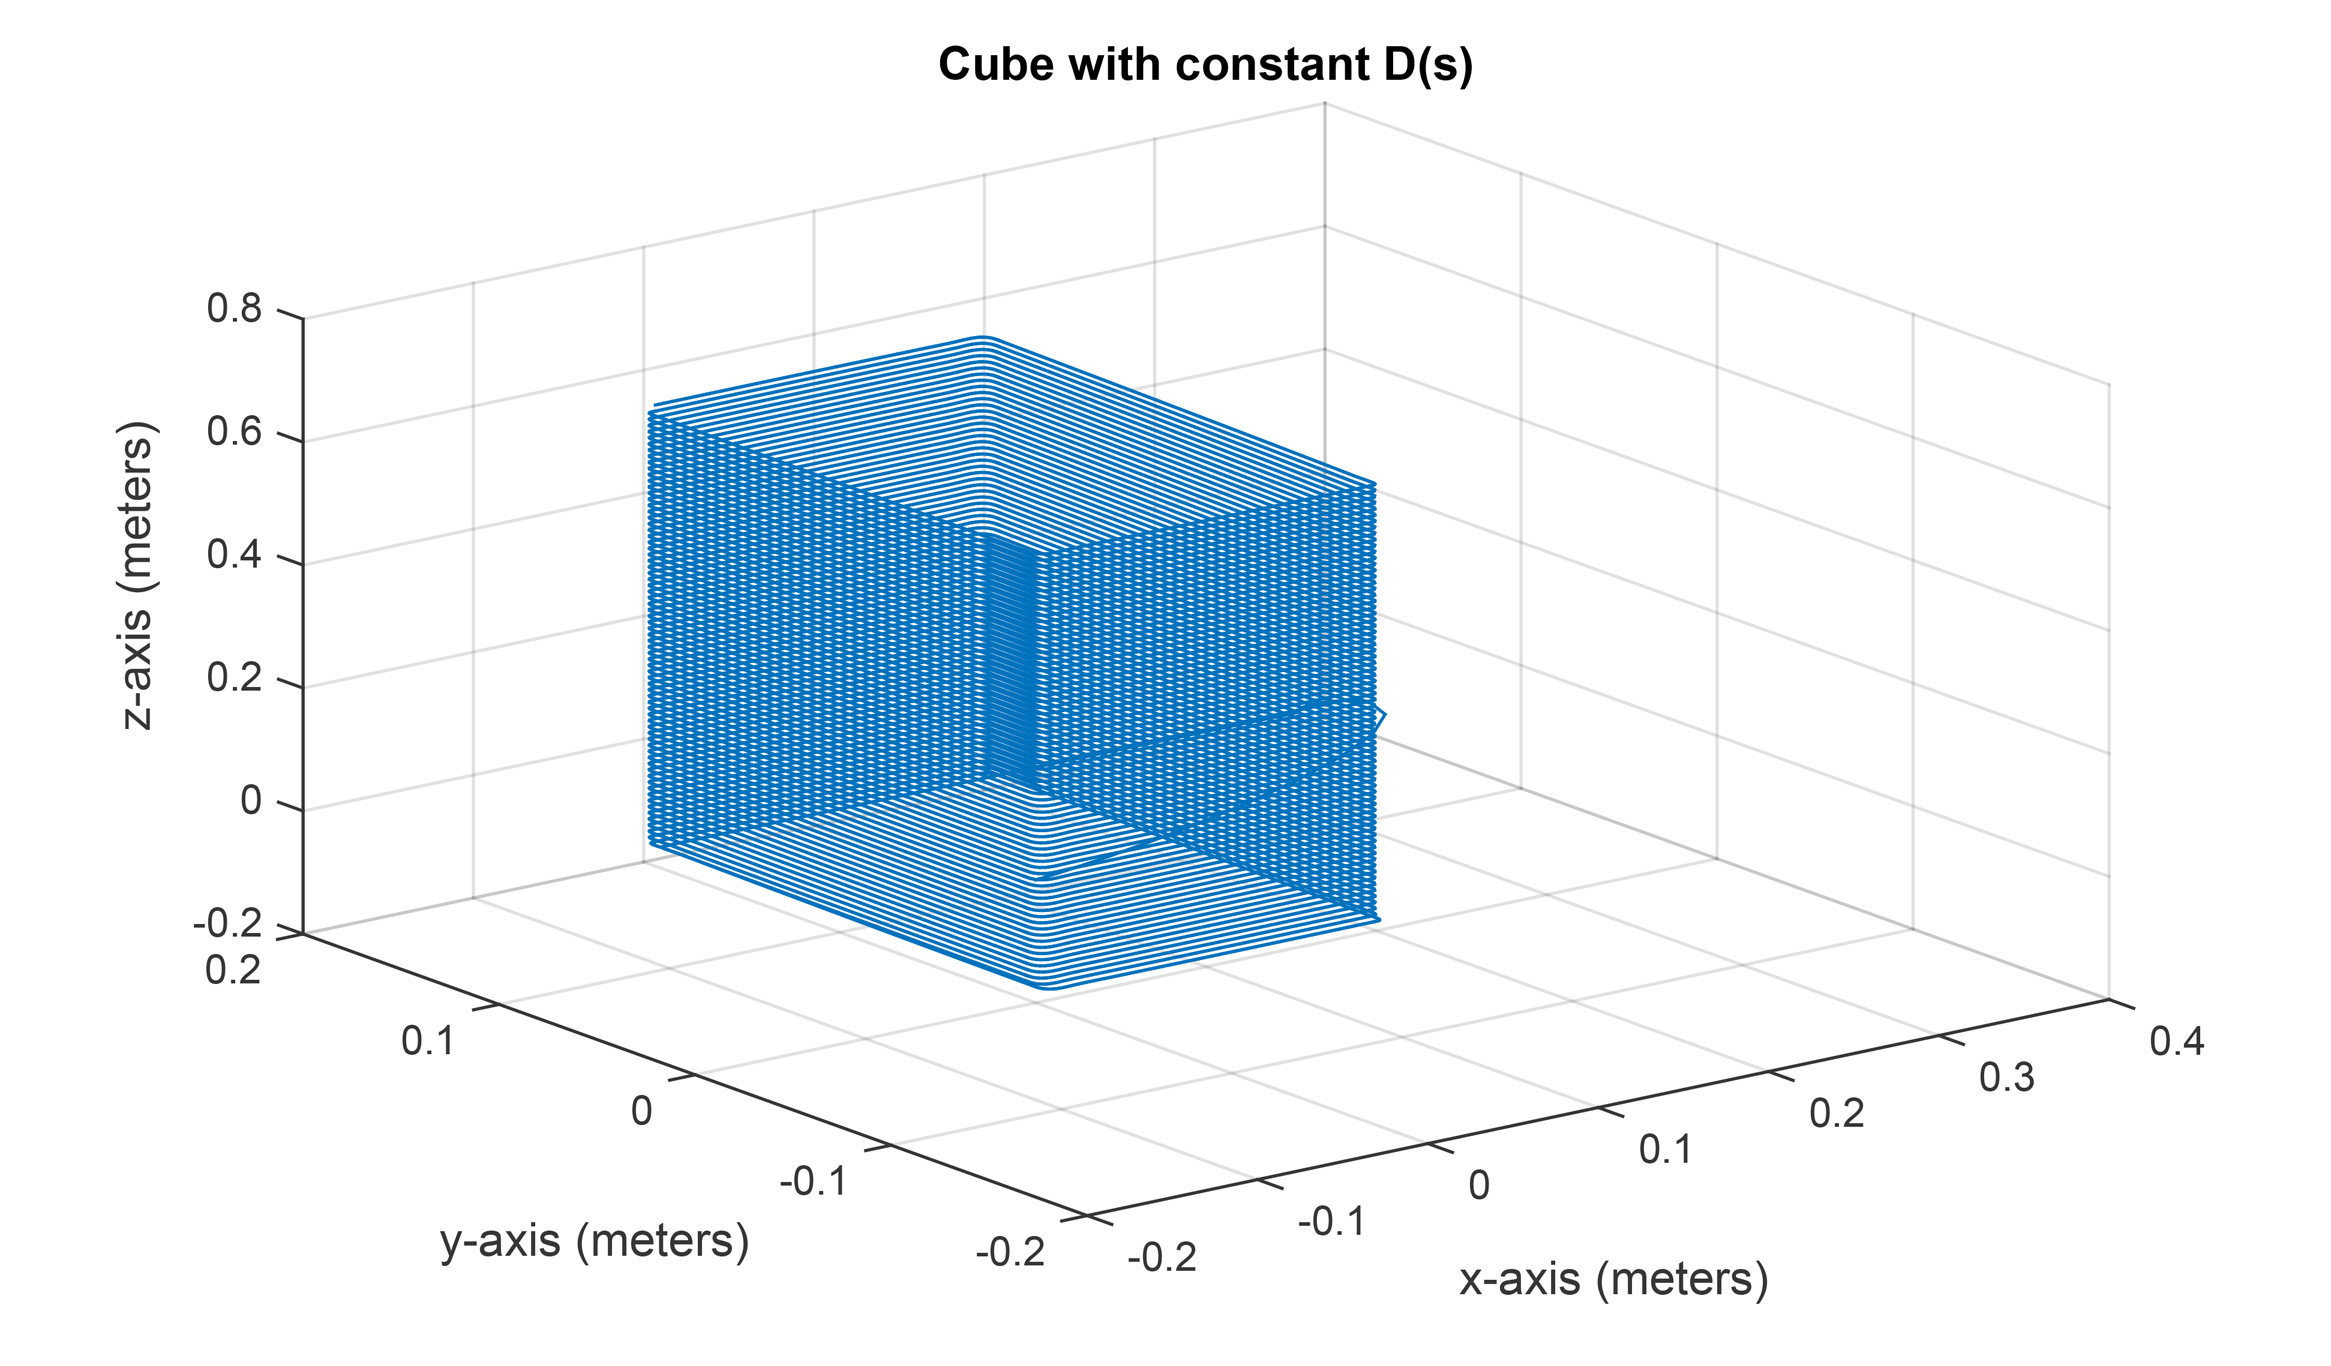
\includegraphics[width=\linewidth]{cube_print_D.pdf}}
\caption{Cube 3d plot without disturbance with D(s)=500N}
\label{fig}
\end{figure}
The edges of Cube is not sharp enough when the figure is zoomed because of error tolerance. The error plots of X, Y and Z motors in case of Cube in shown Fig. 44, Fig. 45 and Fig. 46 respectively. Although error increases with disturbance but was quiet small to produce any visual change in the printed object.
 \begin{figure}[htbp]
\centerline{\includegraphics[width=\linewidth]{cube_errx_D.pdf}}
\caption{X motor error plot while printing Cube with D(s)}
\label{fig}
\end{figure}\begin{figure}[htbp]
\centerline{\includegraphics[width=\linewidth]{cube_erry_D.pdf}}
\caption{Y motor error plot while printing Cube with D(s)}
\label{fig}
\end{figure}\begin{figure}[htbp]
\centerline{\includegraphics[width=\linewidth]{cube_errz_D.pdf}}
\caption{Z motor error plot while printing Cube with D(s)}
\label{fig}
\end{figure}
\subsection{3d printing of Pyramid with D(s)}
The 3d plot of Pyramid shown in Fig. 47 without any disturbance.
\begin{figure}[htbp]
\centerline{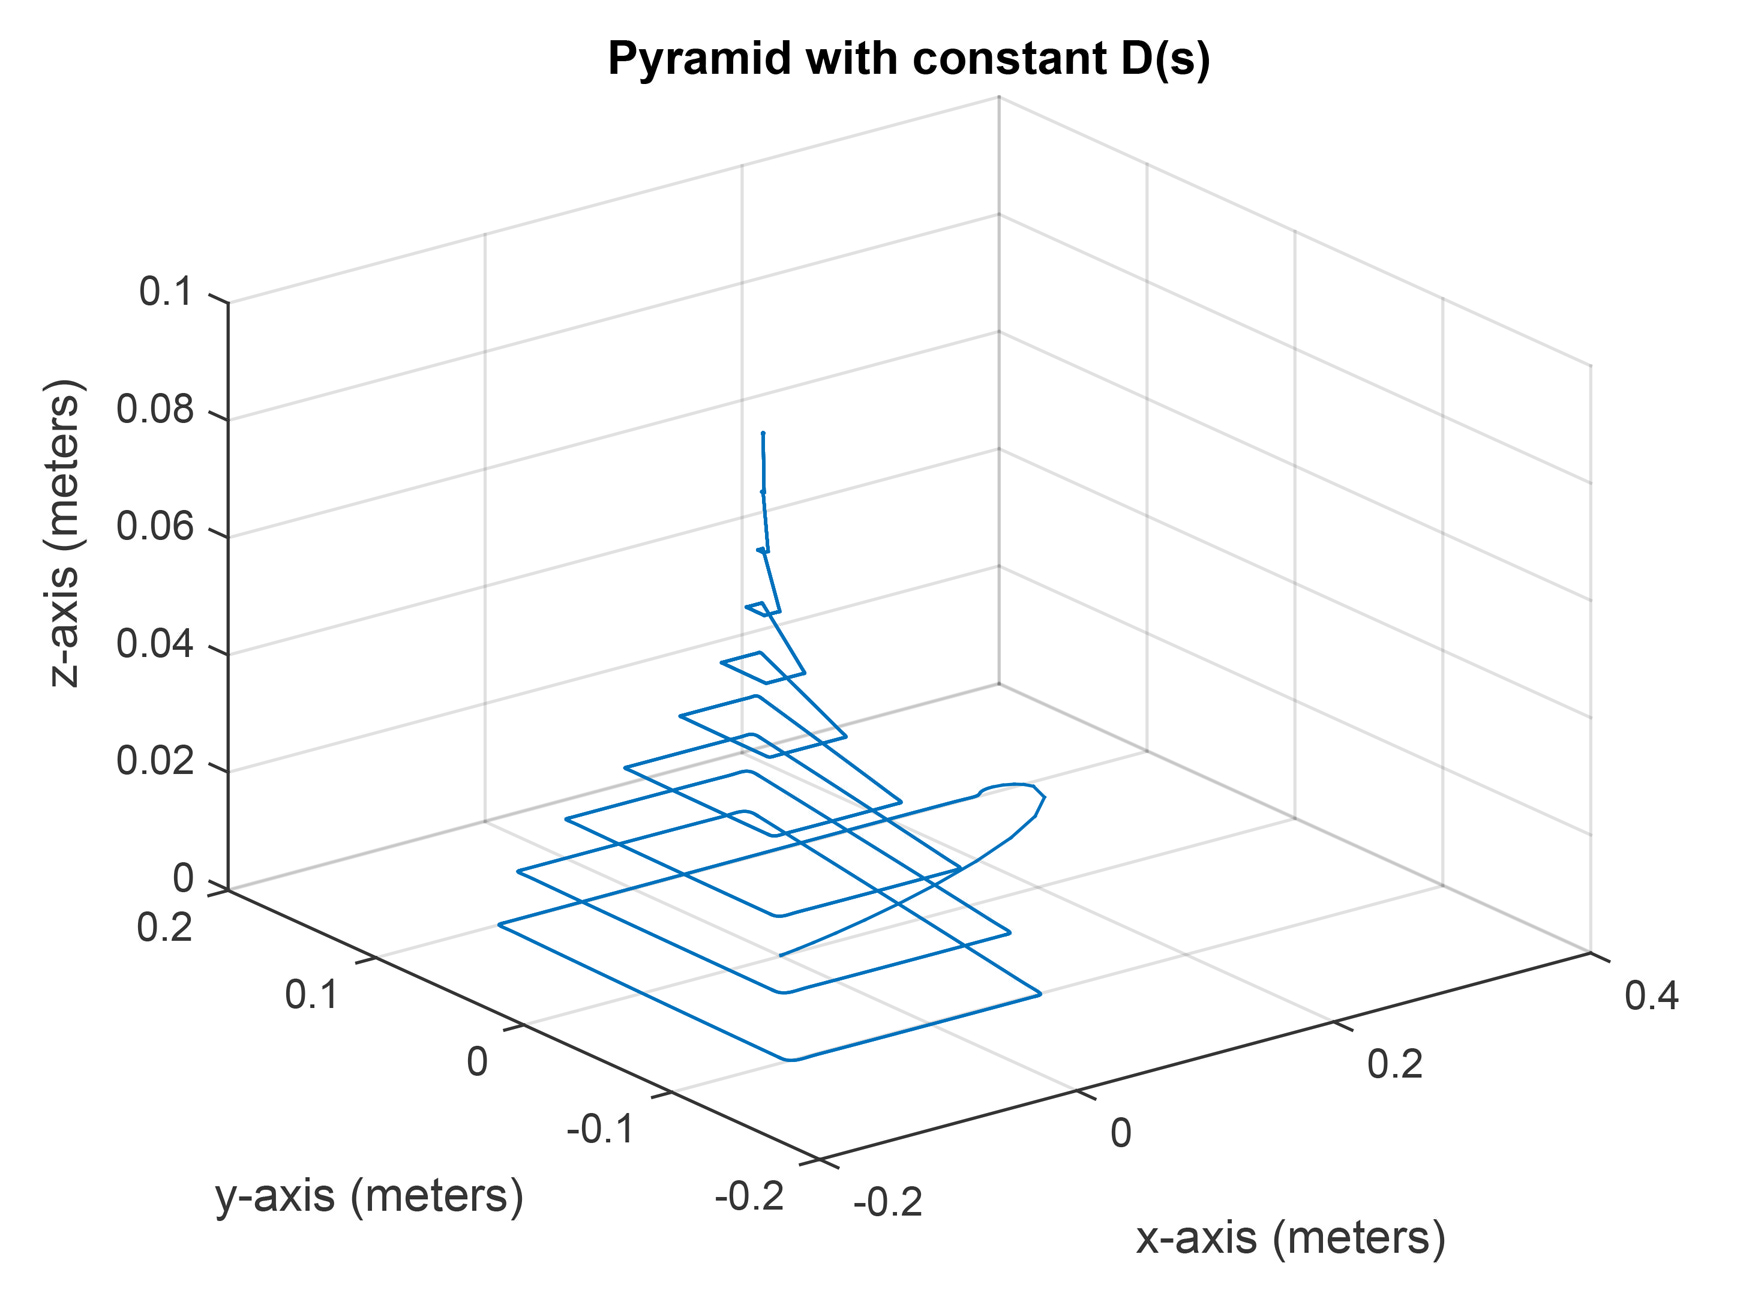
\includegraphics[width=\linewidth]{pyramid_print_D.pdf}}
\caption{Pyramid 3d plot without disturbance with D(s)=500N}
\label{fig}
\end{figure}
The edges of Pyramid is not sharp enough when the figure is zoomed because of error tolerance. The error plots of X, Y and Z motors in case of Pyramid in shown Fig. 48, Fig. 49 and Fig. 50 respectively. Although error increases with disturbance but was quiet small to produce any visual change in the printed object.
 \begin{figure}[htbp]
\centerline{\includegraphics[width=\linewidth]{pyramid_errx_D.pdf}}
\caption{X motor error plot while printing Pyramid with D(s)}
\label{fig}
\end{figure}\begin{figure}[htbp]
\centerline{\includegraphics[width=\linewidth]{pyramid_erry_D.pdf}}
\caption{Y motor error plot while printing Pyramid with D(s)}
\label{fig}
\end{figure}\begin{figure}[htbp]
\centerline{\includegraphics[width=\linewidth]{pyramid_errz_D.pdf}}
\caption{Z motor error plot while printing Pyramid with D(s)}
\label{fig}
\end{figure}
\subsection{Comparative error plots with and without D(s)}
Comparative plots of error of motor X, Y and Z while printing \textbf{Cube} are shown in Fig. 51, Fig 52, Fig. 53. When the disturbance of 500N is applied , the error increases but unable to vary the settling time because of the designed compensator, therefore, slight variation doesn't effect the final printed object.
\begin{figure}[htbp]
\centerline{\includegraphics[width=\linewidth]{dis_X_final.pdf}}
\caption{X motor error plot with and without D(s)}
\label{fig}
\end{figure}\begin{figure}[htbp]
\centerline{\includegraphics[width=\linewidth]{dis_Y_final.pdf}}
\caption{Y motor error plot with and without D(s))}
\label{fig}
\end{figure}\begin{figure}[htbp]
\centerline{\includegraphics[width=\linewidth]{dis_Z_final.pdf}}
\caption{Z motor motor error plot with and without D(s)}
\label{fig}
\end{figure}
\section{Conclusion}
The mathematical modeling of transfer function of X, Y and  Z motors along with its gear and load has been performed. Then a Lead controller has been designed to control each X, Y and Z feedback loop individually. Simulation results proved that the controller can compensate a disturbance of upto 500N which is a quiet large value in terms of 3d printer. Moreover, 3d objects has been printed using designed 3d printer model in simulink by giving input coordinates from pseudo .stl file.

\section*{List of Symbols}\noindent
- $e_m(t)$: motor input voltage\\
- $i_a(t)$ : motor armature current\\
- $L_a,R_a$ : motor armature inductance and resistance\\
- $\tau_m,\theta_m$ : motor side torque and angular position\\
- $\frac{N_2}{N_1}=r$ : gear ratio\\
- $\tau_L,\theta_L$ : load side torque and angular position\\
- $m_L$ : load mass\\
- $x_L(t)$ : load displacement\\
- $b$ : load friction\\
- $f_L(t)$ : lead screw force\\
- $J_m$ : moment of inertia (motor)\\
- $J_p$: moment of inertia (pinion connected to the motor)\\
- $J_{mot}$ : $J_m+J_p$\\
- $J_g$ : moment of inertia (big gear)\\
- $J_s$ : moment of inertial (gear output shaft)\\
- $J_{lod}$ : $J_g+J_s$ \\
- $K_s$ : lead screw power factor \\
- $K_R$ : rotation to linear displacement conversion constant\\
- $D_1$ : motor friction\\
- $D_2$ : gear output shaft friction\\
- $K_t$ : motor torque constant\\
- $K_b$ : motor back emf constant\\

\begin{thebibliography}{00}
\bibitem{b1} Spong, Mark W., and Mathukumalli Vidyasagar. Robot dynamics and control. John Wiley and Sons, 2008.
\end{thebibliography}

\end{document}
